\documentclass[twoside]{book}

% Packages required by doxygen
\usepackage{fixltx2e}
\usepackage{calc}
\usepackage{doxygen}
\usepackage{graphicx}
\usepackage[utf8]{inputenc}
\usepackage{makeidx}
\usepackage{multicol}
\usepackage{multirow}
\PassOptionsToPackage{warn}{textcomp}
\usepackage{textcomp}
\usepackage[nointegrals]{wasysym}
\usepackage[table]{xcolor}

% NLS support packages
\usepackage[spanish]{babel}
% Font selection
\usepackage[T1]{fontenc}
\usepackage{mathptmx}
\usepackage[scaled=.90]{helvet}
\usepackage{courier}
\usepackage{amssymb}
\usepackage{sectsty}
\renewcommand{\familydefault}{\sfdefault}
\allsectionsfont{%
  \fontseries{bc}\selectfont%
  \color{darkgray}%
}
\renewcommand{\DoxyLabelFont}{%
  \fontseries{bc}\selectfont%
  \color{darkgray}%
}
\newcommand{\+}{\discretionary{\mbox{\scriptsize$\hookleftarrow$}}{}{}}

% Page & text layout
\usepackage{geometry}
\geometry{%
  a4paper,%
  top=2.5cm,%
  bottom=2.5cm,%
  left=2.5cm,%
  right=2.5cm%
}
\tolerance=750
\hfuzz=15pt
\hbadness=750
\setlength{\emergencystretch}{15pt}
\setlength{\parindent}{0cm}
\setlength{\parskip}{0.2cm}
\makeatletter
\renewcommand{\paragraph}{%
  \@startsection{paragraph}{4}{0ex}{-1.0ex}{1.0ex}{%
    \normalfont\normalsize\bfseries\SS@parafont%
  }%
}
\renewcommand{\subparagraph}{%
  \@startsection{subparagraph}{5}{0ex}{-1.0ex}{1.0ex}{%
    \normalfont\normalsize\bfseries\SS@subparafont%
  }%
}
\makeatother

% Headers & footers
\usepackage{fancyhdr}
\pagestyle{fancyplain}
\fancyhead[LE]{\fancyplain{}{\bfseries\thepage}}
\fancyhead[CE]{\fancyplain{}{}}
\fancyhead[RE]{\fancyplain{}{\bfseries\leftmark}}
\fancyhead[LO]{\fancyplain{}{\bfseries\rightmark}}
\fancyhead[CO]{\fancyplain{}{}}
\fancyhead[RO]{\fancyplain{}{\bfseries\thepage}}
\fancyfoot[LE]{\fancyplain{}{}}
\fancyfoot[CE]{\fancyplain{}{}}
\fancyfoot[RE]{\fancyplain{}{\bfseries\scriptsize Generado el Viernes, 12 de Diciembre de 2014 11\+:41\+:30 para Documentacion C\+C\+O por Doxygen }}
\fancyfoot[LO]{\fancyplain{}{\bfseries\scriptsize Generado el Viernes, 12 de Diciembre de 2014 11\+:41\+:30 para Documentacion C\+C\+O por Doxygen }}
\fancyfoot[CO]{\fancyplain{}{}}
\fancyfoot[RO]{\fancyplain{}{}}
\renewcommand{\footrulewidth}{0.4pt}
\renewcommand{\chaptermark}[1]{%
  \markboth{#1}{}%
}
\renewcommand{\sectionmark}[1]{%
  \markright{\thesection\ #1}%
}

% Indices & bibliography
\usepackage{natbib}
\usepackage[titles]{tocloft}
\setcounter{tocdepth}{3}
\setcounter{secnumdepth}{5}
\makeindex

% Hyperlinks (required, but should be loaded last)
\usepackage{ifpdf}
\ifpdf
  \usepackage[pdftex,pagebackref=true]{hyperref}
\else
  \usepackage[ps2pdf,pagebackref=true]{hyperref}
\fi
\hypersetup{%
  colorlinks=true,%
  linkcolor=blue,%
  citecolor=blue,%
  unicode%
}

% Custom commands
\newcommand{\clearemptydoublepage}{%
  \newpage{\pagestyle{empty}\cleardoublepage}%
}


%===== C O N T E N T S =====

\begin{document}

% Titlepage & ToC
\hypersetup{pageanchor=false,
             bookmarks=true,
             bookmarksnumbered=true,
             pdfencoding=unicode
            }
\pagenumbering{roman}
\begin{titlepage}
\vspace*{7cm}
\begin{center}%
{\Large Documentacion C\+C\+O }\\
\vspace*{1cm}
{\large Generado por Doxygen 1.8.8}\\
\vspace*{0.5cm}
{\small Viernes, 12 de Diciembre de 2014 11:41:30}\\
\end{center}
\end{titlepage}
\clearemptydoublepage
\tableofcontents
\clearemptydoublepage
\pagenumbering{arabic}
\hypersetup{pageanchor=true}

%--- Begin generated contents ---
\chapter{Documentación de C.\+C.\+O. -\/ Clonal Colony Optimization}
\label{index}\hypertarget{index}{}En la presente documentación, se documentarán los métodos y clases implementadas en la metaheurística C.\+C.\+O. ({\bfseries C}lonal {\bfseries C}olony {\bfseries O}ptmization), que se encuentran codificados en el lenguaje de programación {\bfseries C++}.

El principal objetivo que se desea lograr al implementar la metaheurística adaptativa e inspirada en la naturaleza C.\+C.\+O., es la de hallar soluciones robustas en problemas de optimización, sin incurrir en costos computacionales extras al evaluar la robustez de las soluciones candidatas. Ésto es posible, al imitar el esquema colaborativo de la {\bfseries colonias clonales} presente en la naturaleza.

La estructura básica de la metaheurística C.\+C.\+O., se encuentra constituida por un {\bfseries algoritmo iterativo generacional}, el cual se describe a continuación\+:



Un complemento idóneo a la presente documentación, correspondería a un reporte técnico. La utilidad que nos presentaría un reporte técnico, sería la de permitirnos relacionar a el código implementado, con la lógica de la metaheurística C.\+C.\+O. 
\begin{DoxyItemize}
\item Enlace disponible para el reporte técnico\+: \href{../html2/HTLATEXDocumentacionCCO.html}{\tt Link-\/$>$}  
\end{DoxyItemize}

Por último, esto es parte de un trabajo de tesis realizado para optar al título de Ingeniero Civil en Informática de la \href{www.uach.cl}{\tt Universidad Austral de Chile}, por lo que las personas relacionadas con ésta, son las siguientes\+:

{\bfseries Profesor patrocinante\+:} 
\begin{DoxyItemize}
\item Dr. Ing. Jorge Patricio Maturana Ortíz (\href{http://www.inf.uach.cl/maturana/}{\tt Personal Page-\/$>$})  
\end{DoxyItemize}{\bfseries Alumno tesista\+:} 
\begin{DoxyItemize}
\item Mauricio Alexis Guarda Oñate 
\end{DoxyItemize}
\chapter{C\+C\+O\+P\+E\+R\+M}
\label{md__r_e_a_d_m_e}
\hypertarget{md__r_e_a_d_m_e}{}
Source code of an implementation for clonal colony optimization method on permutations, focused on travell salesman problem and quadratic assignment problem 
\chapter{Lista de tareas pendientes}
\label{todo}
\hypertarget{todo}{}

\begin{DoxyRefList}
\item[\label{todo__todo000001}%
\hypertarget{todo__todo000001}{}%
Member \hyperlink{class_c_c_o_a8b93a09d017497a2a636bd092883f06a}{C\+C\+O\+:\+:Competition} (int const iter)]revisar caso de moneda 
\end{DoxyRefList}
\chapter{Indice jerárquico}
\section{Jerarquía de la clase}
Esta lista de herencias esta ordenada aproximadamente por orden alfabético\+:\begin{DoxyCompactList}
\item \contentsline{section}{C\+C\+O}{\pageref{class_c_c_o}}{}
\item \contentsline{section}{Colony}{\pageref{class_colony}}{}
\item \contentsline{section}{Plant}{\pageref{class_plant}}{}
\item \contentsline{section}{Problem}{\pageref{class_problem}}{}
\begin{DoxyCompactList}
\item \contentsline{section}{Qap}{\pageref{class_qap}}{}
\item \contentsline{section}{Tsp}{\pageref{class_tsp}}{}
\end{DoxyCompactList}
\item \contentsline{section}{rand31dc}{\pageref{classrand31dc}}{}
\item \contentsline{section}{Solution}{\pageref{class_solution}}{}
\begin{DoxyCompactList}
\item \contentsline{section}{Solution\+Perm}{\pageref{class_solution_perm}}{}
\end{DoxyCompactList}
\item \contentsline{section}{toolbox}{\pageref{classtoolbox}}{}
\end{DoxyCompactList}

\chapter{Índice de clases}
\section{Class List}
Here are the classes, structs, unions and interfaces with brief descriptions\+:\begin{DoxyCompactList}
\item\contentsline{section}{\hyperlink{class_c_c_o}{C\+C\+O} \\*\hyperlink{class_c_c_o}{C\+C\+O} (Clonal \hyperlink{class_colony}{Colony} Optimization) }{\pageref{class_c_c_o}}{}
\item\contentsline{section}{\hyperlink{class_colony}{Colony} \\*Clase que gestiona a objetos del tipo \hyperlink{class_plant}{Plant} }{\pageref{class_colony}}{}
\item\contentsline{section}{\hyperlink{class_plant}{Plant} \\*Define los objetos \hyperlink{class_plant}{Plant} }{\pageref{class_plant}}{}
\item\contentsline{section}{\hyperlink{class_problem}{Problem} \\*Clase abstracta \hyperlink{class_problem}{Problem} }{\pageref{class_problem}}{}
\item\contentsline{section}{\hyperlink{class_qap}{Qap} }{\pageref{class_qap}}{}
\item\contentsline{section}{\hyperlink{classrand31dc}{rand31dc} \\*31 bit pseudo-\/random number generator based on Lehmer (1951); Lewis, Goodman \& Miller (1969); Park \& Miller (1983) }{\pageref{classrand31dc}}{}
\item\contentsline{section}{\hyperlink{class_solution}{Solution} \\*Clase Abstracta \hyperlink{class_solution}{Solution} }{\pageref{class_solution}}{}
\item\contentsline{section}{\hyperlink{class_solution_perm}{Solution\+Perm} }{\pageref{class_solution_perm}}{}
\item\contentsline{section}{\hyperlink{classtoolbox}{toolbox} \\*Singleton class (only one object is instantiated) that provides general-\/use methods }{\pageref{classtoolbox}}{}
\item\contentsline{section}{\hyperlink{class_tsp}{Tsp} }{\pageref{class_tsp}}{}
\end{DoxyCompactList}

\chapter{Documentación de las clases}
\hypertarget{class_c_c_o}{\section{C\+C\+O Class Reference}
\label{class_c_c_o}\index{C\+C\+O@{C\+C\+O}}
}


\hyperlink{class_c_c_o}{C\+C\+O} (Clonal \hyperlink{class_colony}{Colony} Optimization)  


\subsection*{Public Member Functions}
\begin{DoxyCompactItemize}
\item 
\hypertarget{class_c_c_o_a48251cd1f851d236c4aec73c82b39682}{\hyperlink{class_c_c_o_a48251cd1f851d236c4aec73c82b39682}{C\+C\+O} ()}\label{class_c_c_o_a48251cd1f851d236c4aec73c82b39682}

\begin{DoxyCompactList}\small\item\em Contructor de la clase \hyperlink{class_c_c_o}{C\+C\+O}. \end{DoxyCompactList}\item 
\hypertarget{class_c_c_o_adaa4d2a9fefa24dfcd6eb8f367f60cf6}{\hyperlink{class_c_c_o_adaa4d2a9fefa24dfcd6eb8f367f60cf6}{$\sim$\+C\+C\+O} ()}\label{class_c_c_o_adaa4d2a9fefa24dfcd6eb8f367f60cf6}

\begin{DoxyCompactList}\small\item\em Destructor de la clase \hyperlink{class_c_c_o}{C\+C\+O}. \end{DoxyCompactList}\item 
void \hyperlink{class_c_c_o_abe96cee0e1a470ea4210ecafe0a4c13e}{run} ()
\begin{DoxyCompactList}\small\item\em Permite ejecutar la clase \hyperlink{class_c_c_o}{C\+C\+O}. \end{DoxyCompactList}\item 
void \hyperlink{class_c_c_o_a611537d0f46ae4573b08a0d8c343da5c}{Purge} (\hyperlink{class_colony}{Colony} $\ast$col, int const iter)
\begin{DoxyCompactList}\small\item\em Metodo que permite eliminar plantas a la colonia. \end{DoxyCompactList}\item 
void \hyperlink{class_c_c_o_a81583df8113bfdd76f5d5d541bdab892}{Extend} (\hyperlink{class_colony}{Colony} $\ast$col, int const iter)
\begin{DoxyCompactList}\small\item\em Metodo que permite agregar plantas a la colonia. \end{DoxyCompactList}\item 
void \hyperlink{class_c_c_o_a5804afdd4b0361d7507fab4b3ab71703}{Split} (\hyperlink{class_colony}{Colony} $\ast$col, int const iter)
\begin{DoxyCompactList}\small\item\em Provoca eventualmente la división de la colonia. \end{DoxyCompactList}\item 
void \hyperlink{class_c_c_o_a8b93a09d017497a2a636bd092883f06a}{Competition} (int const iter)
\begin{DoxyCompactList}\small\item\em Metodo que estimula la competicion de las colonias. \end{DoxyCompactList}\item 
void \hyperlink{class_c_c_o_ae92e0bf5ad45ce36f7e078634e1f42f1}{Distill} ()
\begin{DoxyCompactList}\small\item\em Metodo que determina del patio la(s) solucion(es) mas robusta(s) y de buena calidad (fitness alto) \end{DoxyCompactList}\end{DoxyCompactItemize}


\subsection{Detailed Description}
\hyperlink{class_c_c_o}{C\+C\+O} (Clonal \hyperlink{class_colony}{Colony} Optimization) 

\subsection{Member Function Documentation}
\hypertarget{class_c_c_o_a8b93a09d017497a2a636bd092883f06a}{\index{C\+C\+O@{C\+C\+O}!Competition@{Competition}}
\index{Competition@{Competition}!C\+C\+O@{C\+C\+O}}
\subsubsection[{Competition}]{\setlength{\rightskip}{0pt plus 5cm}void C\+C\+O\+::\+Competition (
\begin{DoxyParamCaption}
\item[{int const}]{iter}
\end{DoxyParamCaption}
)}}\label{class_c_c_o_a8b93a09d017497a2a636bd092883f06a}


Metodo que estimula la competicion de las colonias. 

En este método, se desea poner a prueba la versatilidad de las colonias, ajustándolas a mayores cambios.

Los criterios simplificados en su funcionamiento, son los siguientes\+:


\begin{DoxyItemize}
\item {\bfseries 1.-\/ Reasignación\+:} Para un número total de plantas que se puedan generar en todo el patio (M\+P\+Y), se debe distribuir proporcionalmente para todas sus colonias(\+C\+O\+L)


\item {\bfseries 2.-\/ Superposición y frente de pareto\+:} En la superposición de una colonia, para aquellas que sobrepasan el 50\% de su área y además si su fitness proporcional es menor, está se debe eliminar. Para aquellas que se dominan mutuamente, osea más del 50\% entre ellas, se escoge al azar cuál de éstas se elimina. Para el caso del frente de pareto, se debe eliminar aquella que sea dominada por las demás colonias, con el criterio del fitness promedio de cada colonia 
\end{DoxyItemize}


\begin{DoxyParams}{Parameters}
{\em iter} & Número de la iteración actual \\
\hline
\end{DoxyParams}
\begin{DoxyRefDesc}{Todo}
\item[\hyperlink{todo__todo000001}{Todo}]revisar caso de moneda \end{DoxyRefDesc}
\hypertarget{class_c_c_o_ae92e0bf5ad45ce36f7e078634e1f42f1}{\index{C\+C\+O@{C\+C\+O}!Distill@{Distill}}
\index{Distill@{Distill}!C\+C\+O@{C\+C\+O}}
\subsubsection[{Distill}]{\setlength{\rightskip}{0pt plus 5cm}void C\+C\+O\+::\+Distill (
\begin{DoxyParamCaption}
{}
\end{DoxyParamCaption}
)}}\label{class_c_c_o_ae92e0bf5ad45ce36f7e078634e1f42f1}


Metodo que determina del patio la(s) solucion(es) mas robusta(s) y de buena calidad (fitness alto) 

Este método determina el o los individuos que posean soluciones robustas y de buena calidad. Ofreciéndole al usuario resultados concretos a su problema.

La o las soluciones que se determinen, son aquellas que pertenecen al {\bfseries frente de Pareto}.

Los criterios que se analizan en el frente de Pareto, son 2, y a continuación se mencionan\+:


\begin{DoxyItemize}
\item {\bfseries 1.-\/} Por cada colonia, se escoge la planta que esté más al centro de ésta. La candidata es aquella planta que tenga la menor suma de distancias a otras plantas de la misma colonia


\item {\bfseries 2.-\/} La robustez, se determina a partir de la división entre el área de la colonia y la varianza de los fitness de todas las plantas de la colonia 
\end{DoxyItemize}

En resumen, la identificación de las soluciones se realiza al finalizar el proceso de la búsqueda y son aquellas que maximizan los criterios anteriormente mencionados, robustez y muy buena calidad. \hypertarget{class_c_c_o_a81583df8113bfdd76f5d5d541bdab892}{\index{C\+C\+O@{C\+C\+O}!Extend@{Extend}}
\index{Extend@{Extend}!C\+C\+O@{C\+C\+O}}
\subsubsection[{Extend}]{\setlength{\rightskip}{0pt plus 5cm}void C\+C\+O\+::\+Extend (
\begin{DoxyParamCaption}
\item[{{\bf Colony} $\ast$}]{colonia, }
\item[{int const}]{iter}
\end{DoxyParamCaption}
)}}\label{class_c_c_o_a81583df8113bfdd76f5d5d541bdab892}


Metodo que permite agregar plantas a la colonia. 

El criterio que determina la planta a extender, se le añade un hijo en su vecindad, de tal modo que quede a una distancia prudente, es decir, ni tan lejos, ni tan cerca de la planta padre.

Los pasos simplificados son los siguientes\+: 
\begin{DoxyItemize}
\item Se escoge una planta (que se llamará aquí \char`\"{}padre\char`\"{}) con el método roullete, sobre la colonia 
\item Se crea una nueva solución, a partir de la planta padre 
\item La nueva solución se extiende 
\item La nueva solución se le agrega a una nueva planta hija 
\item La nueva planta hija se agrega a la planta padre 
\end{DoxyItemize}


\begin{DoxyParams}{Parameters}
{\em colonia$\ast$} & Puntero a la colonia que se añadirá una planta. \\
\hline
{\em iter} & Número de la iteración actual \\
\hline
\end{DoxyParams}
\hypertarget{class_c_c_o_a611537d0f46ae4573b08a0d8c343da5c}{\index{C\+C\+O@{C\+C\+O}!Purge@{Purge}}
\index{Purge@{Purge}!C\+C\+O@{C\+C\+O}}
\subsubsection[{Purge}]{\setlength{\rightskip}{0pt plus 5cm}void C\+C\+O\+::\+Purge (
\begin{DoxyParamCaption}
\item[{{\bf Colony} $\ast$}]{colonia, }
\item[{int const}]{iter}
\end{DoxyParamCaption}
)}}\label{class_c_c_o_a611537d0f46ae4573b08a0d8c343da5c}


Metodo que permite eliminar plantas a la colonia. 

El criterio que determina la planta a eliminar, es para aquella que posea el peor fitness de la colonia.

Los pasos simplificados son los siguientes\+: 
\begin{DoxyItemize}
\item Se escoge la planta que tenga el peor fitness de la colonia 
\item Se elimina la planta, modificando así a la colonia 
\end{DoxyItemize}


\begin{DoxyParams}{Parameters}
{\em colonia$\ast$} & Puntero a la colonia que se le eliminará una planta. \\
\hline
{\em iter} & Número de la iteración actual \\
\hline
\end{DoxyParams}
\hypertarget{class_c_c_o_abe96cee0e1a470ea4210ecafe0a4c13e}{\index{C\+C\+O@{C\+C\+O}!run@{run}}
\index{run@{run}!C\+C\+O@{C\+C\+O}}
\subsubsection[{run}]{\setlength{\rightskip}{0pt plus 5cm}void C\+C\+O\+::run (
\begin{DoxyParamCaption}
{}
\end{DoxyParamCaption}
)}}\label{class_c_c_o_abe96cee0e1a470ea4210ecafe0a4c13e}


Permite ejecutar la clase \hyperlink{class_c_c_o}{C\+C\+O}. 

En este método se implementa toda la {\bfseries lógica de la metaheurística}, que coordina las interacciones entre las clases \hyperlink{class_plant}{Plant} y \hyperlink{class_colony}{Colony}.

Los pasos simplificados son los siguientes\+: 
\begin{DoxyCode}
While\{ejecutar las MAXGEN iteraciones\}\{

    ForEach\{colonia en el patio\}\{
        \hyperlink{class_c_c_o_a611537d0f46ae4573b08a0d8c343da5c}{Purge}(colonia)
        \hyperlink{class_c_c_o_a81583df8113bfdd76f5d5d541bdab892}{Extend}(colonia)
        \hyperlink{class_c_c_o_a5804afdd4b0361d7507fab4b3ab71703}{Split}(colonia)
 \}

    \hyperlink{class_c_c_o_a8b93a09d017497a2a636bd092883f06a}{Competition}()
\}

\hyperlink{class_c_c_o_ae92e0bf5ad45ce36f7e078634e1f42f1}{Distill}()
\end{DoxyCode}
 \hypertarget{class_c_c_o_a5804afdd4b0361d7507fab4b3ab71703}{\index{C\+C\+O@{C\+C\+O}!Split@{Split}}
\index{Split@{Split}!C\+C\+O@{C\+C\+O}}
\subsubsection[{Split}]{\setlength{\rightskip}{0pt plus 5cm}void C\+C\+O\+::\+Split (
\begin{DoxyParamCaption}
\item[{{\bf Colony} $\ast$}]{colonia, }
\item[{int const}]{iter}
\end{DoxyParamCaption}
)}}\label{class_c_c_o_a5804afdd4b0361d7507fab4b3ab71703}


Provoca eventualmente la división de la colonia. 

El criterio que determina las plantas a cortar, es para una distancia lo suficientemente larga y que a lo menos exista en sus extremos 3 plantas por lado, se procede a cortarlas y/o liberarlas.

Las plantas cortadas de la colonia inicial, son tratadas como una nueva colonia en el patio, con la primera planta ubicada en el extremo de la mayor distancia, como la planta raíz (root) de la nueva colonia.

Los pasos simplificados son los siguientes\+: 
\begin{DoxyItemize}
\item Encontrar la distancia que satisface el criterio de corte entre las plantas de la colonia 
\item Se crea una nueva colonia 
\item Se establece la primera planta del extremo, como la raíz (root) de la nueva colonia 
\item La nueva colonia se agrega al patio 
\end{DoxyItemize}


\begin{DoxyParams}{Parameters}
{\em colonia$\ast$} & Puntero a la colonia que se le aplicará o no un corte. \\
\hline
{\em iter} & Número de la iteración actual \\
\hline
\end{DoxyParams}


The documentation for this class was generated from the following files\+:\begin{DoxyCompactItemize}
\item 
B\+A\+S\+E/cco.\+h\item 
B\+A\+S\+E/cco.\+cpp\end{DoxyCompactItemize}

\hypertarget{class_colony}{\section{Colony Class Reference}
\label{class_colony}\index{Colony@{Colony}}
}


Clase que gestiona a objetos del tipo \hyperlink{class_plant}{Plant}.  


\subsection*{Public Member Functions}
\begin{DoxyCompactItemize}
\item 
\hypertarget{class_colony_aaf760edad97dee7263b86913d3bb4f98}{\hyperlink{class_colony_aaf760edad97dee7263b86913d3bb4f98}{Colony} ()}\label{class_colony_aaf760edad97dee7263b86913d3bb4f98}

\begin{DoxyCompactList}\small\item\em Constructor de la clase. \end{DoxyCompactList}\item 
\hypertarget{class_colony_a9cebe4a25260c8da7c99d10b0dab5a4e}{\hyperlink{class_colony_a9cebe4a25260c8da7c99d10b0dab5a4e}{$\sim$\+Colony} ()}\label{class_colony_a9cebe4a25260c8da7c99d10b0dab5a4e}

\begin{DoxyCompactList}\small\item\em Destructor de la clase. \end{DoxyCompactList}\item 
void \hyperlink{class_colony_a23cb5efacc701479fb4cfdb3cfd5fdc5}{set\+\_\+root} (\hyperlink{class_plant}{Plant} $\ast$const)
\begin{DoxyCompactList}\small\item\em Establece a la planta raíz de la colonia. \end{DoxyCompactList}\item 
\hyperlink{class_plant}{Plant} $\ast$ \hyperlink{class_colony_afb7f538de55475561a46f8d4c2c65c8b}{get\+\_\+root} () const 
\begin{DoxyCompactList}\small\item\em Retorna el puntero a la planta raíz. \end{DoxyCompactList}\item 
void \hyperlink{class_colony_a29b64da9f582127b41616466c0b6232c}{set\+Name} (string nombre)
\begin{DoxyCompactList}\small\item\em Establece el nombre de la actual colonia. \end{DoxyCompactList}\item 
string \hyperlink{class_colony_aeb93331a87786184e3373f63ab643462}{get\+Name} ()
\begin{DoxyCompactList}\small\item\em Retorna el nombre asignado a la colonia. \end{DoxyCompactList}\item 
void \hyperlink{class_colony_ac31cfb633a10ab2e348d6a1a927c68d9}{set\+M\+P\+C} (int)
\begin{DoxyCompactList}\small\item\em Establecer el número de plantas que puede poseer la colonia (M\+P\+C) \end{DoxyCompactList}\item 
double \hyperlink{class_colony_a73d51b415918b9f0f123240a6f2101b5}{get\+M\+P\+C} () const 
\begin{DoxyCompactList}\small\item\em Retorna el número de plantas que puede poseer la colonia (M\+P\+C) \end{DoxyCompactList}\item 
\hyperlink{class_plant}{Plant} $\ast$ \hyperlink{class_colony_ac47cd3350e58715470ebadbf0a0e4eaf}{replace\+\_\+root} (\hyperlink{class_plant}{Plant} $\ast$const addr)
\begin{DoxyCompactList}\small\item\em Establece el reemplazante de la raíz. \end{DoxyCompactList}\item 
int \hyperlink{class_colony_a9f647ee71e990d77daeb95a72d2251ec}{get\+Size} () const 
\begin{DoxyCompactList}\small\item\em Retorna el tamaño de la colonia. \end{DoxyCompactList}\item 
\hyperlink{class_plant}{Plant} $\ast$ \hyperlink{class_colony_a686417d078d3544d7c07309822a8c45e}{get\+Best\+Plant} ()
\begin{DoxyCompactList}\small\item\em Retorna la planta de mayor fitness. \end{DoxyCompactList}\item 
\hyperlink{class_plant}{Plant} $\ast$ \hyperlink{class_colony_a858397bdf56c10bdc8035f907b0d227e}{get\+Worst\+Plant} ()
\begin{DoxyCompactList}\small\item\em Retorna la planta de menor fitness. \end{DoxyCompactList}\item 
std\+::list$<$ \hyperlink{class_plant}{Plant} $\ast$ $>$ \hyperlink{class_colony_a349e5b625a4f62dd55a3911319051df7}{get\+Plants} ()
\begin{DoxyCompactList}\small\item\em Retorna las plantas de la colonia. \end{DoxyCompactList}\item 
\hypertarget{class_colony_a768a1fa3225bce6b7c28031d0efac929}{void \hyperlink{class_colony_a768a1fa3225bce6b7c28031d0efac929}{update\+\_\+\+T\+Fitness} ()}\label{class_colony_a768a1fa3225bce6b7c28031d0efac929}

\begin{DoxyCompactList}\small\item\em Actualizar el T\+Fitness para la colonia. \end{DoxyCompactList}\item 
double \hyperlink{class_colony_a396ffff8734870bb149f6205eede5443}{get\+Mean\+Colony} () const 
\begin{DoxyCompactList}\small\item\em Retorna el promedio de Fitness de la colonia. \end{DoxyCompactList}\item 
\hyperlink{class_plant}{Plant} $\ast$ \hyperlink{class_colony_a095984a4b9d66dccd04512f77b70fbe9}{roulette} ()
\begin{DoxyCompactList}\small\item\em Escoge al azar una Planta de la colonia. \end{DoxyCompactList}\item 
double \hyperlink{class_colony_adaa8bc27180fe9b61656acb6185250b7}{get\+Area} ()
\begin{DoxyCompactList}\small\item\em Retorna el area de la colonia. \end{DoxyCompactList}\item 
double \hyperlink{class_colony_ac985894236686089847cc80eef0df3c0}{get\+Varianza} ()
\begin{DoxyCompactList}\small\item\em Retorna la varianza de la colonia con respecto al Fitness de las plantas. \end{DoxyCompactList}\item 
double \hyperlink{class_colony_ac59ef383ec4d254fef1326b33812fd66}{get\+Min\+Value} (int dimension)
\begin{DoxyCompactList}\small\item\em Retorna la menor coordenada de la colonia. \end{DoxyCompactList}\item 
double \hyperlink{class_colony_a177a36f388719982d16c2abcacef85a3}{get\+Max\+Value} (int dimension)
\begin{DoxyCompactList}\small\item\em Retorna la mayor coordenada de la colonia. \end{DoxyCompactList}\item 
double \hyperlink{class_colony_a7f27439201f57d52df38115c10f41bf2}{Superposicion} (\hyperlink{class_colony}{Colony} $\ast$col2)
\begin{DoxyCompactList}\small\item\em Retorna el area de intersección con respecto a otra colonia. \end{DoxyCompactList}\item 
\hyperlink{class_plant}{Plant} $\ast$ \hyperlink{class_colony_a911588b5aab6106b94e9a039ffd61060}{get\+Old\+Plant} ()
\begin{DoxyCompactList}\small\item\em Retorna la planta mas antigua. \end{DoxyCompactList}\item 
\hypertarget{class_colony_add10150a1003dbf88bd9e878509b5367}{void \hyperlink{class_colony_add10150a1003dbf88bd9e878509b5367}{change\+\_\+colony} ()}\label{class_colony_add10150a1003dbf88bd9e878509b5367}

\begin{DoxyCompactList}\small\item\em Establece la colonia actual. \end{DoxyCompactList}\item 
\hyperlink{class_plant}{Plant} $\ast$ \hyperlink{class_colony_a665b63676510d72cc12d4a658f795dff}{Split} (int tam, double max\+\_\+dist)
\begin{DoxyCompactList}\small\item\em Split para la colonia. \end{DoxyCompactList}\item 
\hyperlink{class_plant}{Plant} $\ast$ \hyperlink{class_colony_a8ce65c7c0abc9edee880ff6275b51e6f}{Purge} ()
\begin{DoxyCompactList}\small\item\em Purge para la colonia. \end{DoxyCompactList}\item 
\hypertarget{class_colony_a5a8aa21bceba4eb522333bbb964a7563}{void \hyperlink{class_colony_a5a8aa21bceba4eb522333bbb964a7563}{Re\+\_\+\+Eval\+\_\+\+Func} ()}\label{class_colony_a5a8aa21bceba4eb522333bbb964a7563}

\begin{DoxyCompactList}\small\item\em Re-\/evaluacion de todos los fitness las plantas de la colonia. \end{DoxyCompactList}\item 
\hypertarget{class_colony_a6a6528cacc995800e343298f3a10715f}{void \hyperlink{class_colony_a6a6528cacc995800e343298f3a10715f}{show\+\_\+colony} ()}\label{class_colony_a6a6528cacc995800e343298f3a10715f}

\begin{DoxyCompactList}\small\item\em despliega el contenido de la colonia \end{DoxyCompactList}\item 
void \hyperlink{class_colony_a9b1ac80bb274d2f8b90e592d11a4894b}{show\+\_\+plot} (int)
\begin{DoxyCompactList}\small\item\em Metodo que permite desplegar grafica de la colonia. \end{DoxyCompactList}\end{DoxyCompactItemize}


\subsection{Detailed Description}
Clase que gestiona a objetos del tipo \hyperlink{class_plant}{Plant}. 

\subsection{Member Function Documentation}
\hypertarget{class_colony_afb7f538de55475561a46f8d4c2c65c8b}{\index{Colony@{Colony}!get\+\_\+root@{get\+\_\+root}}
\index{get\+\_\+root@{get\+\_\+root}!Colony@{Colony}}
\subsubsection[{get\+\_\+root}]{\setlength{\rightskip}{0pt plus 5cm}{\bf Plant} $\ast$ Colony\+::get\+\_\+root (
\begin{DoxyParamCaption}
{}
\end{DoxyParamCaption}
) const}}\label{class_colony_afb7f538de55475561a46f8d4c2c65c8b}


Retorna el puntero a la planta raíz. 

\begin{DoxyReturn}{Returns}
Retorna puntero del tipo \hyperlink{class_plant}{Plant}, con la planta raíz de la colonia 
\end{DoxyReturn}
\hypertarget{class_colony_adaa8bc27180fe9b61656acb6185250b7}{\index{Colony@{Colony}!get\+Area@{get\+Area}}
\index{get\+Area@{get\+Area}!Colony@{Colony}}
\subsubsection[{get\+Area}]{\setlength{\rightskip}{0pt plus 5cm}double Colony\+::get\+Area (
\begin{DoxyParamCaption}
{}
\end{DoxyParamCaption}
)}}\label{class_colony_adaa8bc27180fe9b61656acb6185250b7}


Retorna el area de la colonia. 

\begin{DoxyReturn}{Returns}
Retorna un valor del tipo double, con el área de la colonia que utiliza en el espacio de búsqueda 
\end{DoxyReturn}
\hypertarget{class_colony_a686417d078d3544d7c07309822a8c45e}{\index{Colony@{Colony}!get\+Best\+Plant@{get\+Best\+Plant}}
\index{get\+Best\+Plant@{get\+Best\+Plant}!Colony@{Colony}}
\subsubsection[{get\+Best\+Plant}]{\setlength{\rightskip}{0pt plus 5cm}{\bf Plant} $\ast$ Colony\+::get\+Best\+Plant (
\begin{DoxyParamCaption}
{}
\end{DoxyParamCaption}
)}}\label{class_colony_a686417d078d3544d7c07309822a8c45e}


Retorna la planta de mayor fitness. 

\begin{DoxyReturn}{Returns}
Retorna un puntero del tipo \hyperlink{class_plant}{Plant}, con la planta de mayor fitness de la colonia 
\end{DoxyReturn}
\hypertarget{class_colony_a177a36f388719982d16c2abcacef85a3}{\index{Colony@{Colony}!get\+Max\+Value@{get\+Max\+Value}}
\index{get\+Max\+Value@{get\+Max\+Value}!Colony@{Colony}}
\subsubsection[{get\+Max\+Value}]{\setlength{\rightskip}{0pt plus 5cm}double Colony\+::get\+Max\+Value (
\begin{DoxyParamCaption}
\item[{int}]{dimension}
\end{DoxyParamCaption}
)}}\label{class_colony_a177a36f388719982d16c2abcacef85a3}


Retorna la mayor coordenada de la colonia. 


\begin{DoxyParams}{Parameters}
{\em dimension} & Valor de la coordenada a analizar\\
\hline
\end{DoxyParams}
\begin{DoxyReturn}{Returns}
Retorna valor del tipo double, con el máximo valor para esa coordenada 
\end{DoxyReturn}
\hypertarget{class_colony_a396ffff8734870bb149f6205eede5443}{\index{Colony@{Colony}!get\+Mean\+Colony@{get\+Mean\+Colony}}
\index{get\+Mean\+Colony@{get\+Mean\+Colony}!Colony@{Colony}}
\subsubsection[{get\+Mean\+Colony}]{\setlength{\rightskip}{0pt plus 5cm}double Colony\+::get\+Mean\+Colony (
\begin{DoxyParamCaption}
{}
\end{DoxyParamCaption}
) const}}\label{class_colony_a396ffff8734870bb149f6205eede5443}


Retorna el promedio de Fitness de la colonia. 

\begin{DoxyReturn}{Returns}
Retorna una valor del tipo double, con el promedio de los fitness de la colonia 
\end{DoxyReturn}
\hypertarget{class_colony_ac59ef383ec4d254fef1326b33812fd66}{\index{Colony@{Colony}!get\+Min\+Value@{get\+Min\+Value}}
\index{get\+Min\+Value@{get\+Min\+Value}!Colony@{Colony}}
\subsubsection[{get\+Min\+Value}]{\setlength{\rightskip}{0pt plus 5cm}double Colony\+::get\+Min\+Value (
\begin{DoxyParamCaption}
\item[{int}]{dimension}
\end{DoxyParamCaption}
)}}\label{class_colony_ac59ef383ec4d254fef1326b33812fd66}


Retorna la menor coordenada de la colonia. 


\begin{DoxyParams}{Parameters}
{\em dimension} & Valor de la coordenada a analizar\\
\hline
\end{DoxyParams}
\begin{DoxyReturn}{Returns}
Retorna valor del tipo double, con el mínimo valor para esa coordenada 
\end{DoxyReturn}
\hypertarget{class_colony_a73d51b415918b9f0f123240a6f2101b5}{\index{Colony@{Colony}!get\+M\+P\+C@{get\+M\+P\+C}}
\index{get\+M\+P\+C@{get\+M\+P\+C}!Colony@{Colony}}
\subsubsection[{get\+M\+P\+C}]{\setlength{\rightskip}{0pt plus 5cm}double Colony\+::get\+M\+P\+C (
\begin{DoxyParamCaption}
{}
\end{DoxyParamCaption}
) const}}\label{class_colony_a73d51b415918b9f0f123240a6f2101b5}


Retorna el número de plantas que puede poseer la colonia (M\+P\+C) 

\begin{DoxyReturn}{Returns}
Retorna un double, con el número de plantas que puede contener la colonia 
\end{DoxyReturn}
\hypertarget{class_colony_aeb93331a87786184e3373f63ab643462}{\index{Colony@{Colony}!get\+Name@{get\+Name}}
\index{get\+Name@{get\+Name}!Colony@{Colony}}
\subsubsection[{get\+Name}]{\setlength{\rightskip}{0pt plus 5cm}string Colony\+::get\+Name (
\begin{DoxyParamCaption}
{}
\end{DoxyParamCaption}
)}}\label{class_colony_aeb93331a87786184e3373f63ab643462}


Retorna el nombre asignado a la colonia. 

\begin{DoxyReturn}{Returns}
Retorna un string, con el nombre de la colonia 
\end{DoxyReturn}
\hypertarget{class_colony_a911588b5aab6106b94e9a039ffd61060}{\index{Colony@{Colony}!get\+Old\+Plant@{get\+Old\+Plant}}
\index{get\+Old\+Plant@{get\+Old\+Plant}!Colony@{Colony}}
\subsubsection[{get\+Old\+Plant}]{\setlength{\rightskip}{0pt plus 5cm}{\bf Plant} $\ast$ Colony\+::get\+Old\+Plant (
\begin{DoxyParamCaption}
{}
\end{DoxyParamCaption}
)}}\label{class_colony_a911588b5aab6106b94e9a039ffd61060}


Retorna la planta mas antigua. 

\begin{DoxyReturn}{Returns}
Retorna puntero del tipo \hyperlink{class_plant}{Plant}, con la planta más antigua de la colonia 
\end{DoxyReturn}
\hypertarget{class_colony_a349e5b625a4f62dd55a3911319051df7}{\index{Colony@{Colony}!get\+Plants@{get\+Plants}}
\index{get\+Plants@{get\+Plants}!Colony@{Colony}}
\subsubsection[{get\+Plants}]{\setlength{\rightskip}{0pt plus 5cm}list$<$ {\bf Plant} $\ast$ $>$ Colony\+::get\+Plants (
\begin{DoxyParamCaption}
{}
\end{DoxyParamCaption}
)}}\label{class_colony_a349e5b625a4f62dd55a3911319051df7}


Retorna las plantas de la colonia. 

\begin{DoxyReturn}{Returns}
Retorna una lista de punteros del tipo \hyperlink{class_plant}{Plant}, con todas las plantas que pertenecen a la colonia 
\end{DoxyReturn}
\hypertarget{class_colony_a9f647ee71e990d77daeb95a72d2251ec}{\index{Colony@{Colony}!get\+Size@{get\+Size}}
\index{get\+Size@{get\+Size}!Colony@{Colony}}
\subsubsection[{get\+Size}]{\setlength{\rightskip}{0pt plus 5cm}int Colony\+::get\+Size (
\begin{DoxyParamCaption}
{}
\end{DoxyParamCaption}
) const}}\label{class_colony_a9f647ee71e990d77daeb95a72d2251ec}


Retorna el tamaño de la colonia. 

\begin{DoxyReturn}{Returns}
Retorna un int, con el tamaño de la colonia 
\end{DoxyReturn}
\hypertarget{class_colony_ac985894236686089847cc80eef0df3c0}{\index{Colony@{Colony}!get\+Varianza@{get\+Varianza}}
\index{get\+Varianza@{get\+Varianza}!Colony@{Colony}}
\subsubsection[{get\+Varianza}]{\setlength{\rightskip}{0pt plus 5cm}double Colony\+::get\+Varianza (
\begin{DoxyParamCaption}
{}
\end{DoxyParamCaption}
)}}\label{class_colony_ac985894236686089847cc80eef0df3c0}


Retorna la varianza de la colonia con respecto al Fitness de las plantas. 

\begin{DoxyReturn}{Returns}
Retorna valor del tipo double, con la varianza de la colonia 
\end{DoxyReturn}
\hypertarget{class_colony_a858397bdf56c10bdc8035f907b0d227e}{\index{Colony@{Colony}!get\+Worst\+Plant@{get\+Worst\+Plant}}
\index{get\+Worst\+Plant@{get\+Worst\+Plant}!Colony@{Colony}}
\subsubsection[{get\+Worst\+Plant}]{\setlength{\rightskip}{0pt plus 5cm}{\bf Plant} $\ast$ Colony\+::get\+Worst\+Plant (
\begin{DoxyParamCaption}
{}
\end{DoxyParamCaption}
)}}\label{class_colony_a858397bdf56c10bdc8035f907b0d227e}


Retorna la planta de menor fitness. 

\begin{DoxyReturn}{Returns}
Retorna puntero del tipo \hyperlink{class_plant}{Plant}, con la planta de peor fitness de la colonia 
\end{DoxyReturn}
\hypertarget{class_colony_a8ce65c7c0abc9edee880ff6275b51e6f}{\index{Colony@{Colony}!Purge@{Purge}}
\index{Purge@{Purge}!Colony@{Colony}}
\subsubsection[{Purge}]{\setlength{\rightskip}{0pt plus 5cm}{\bf Plant} $\ast$ Colony\+::\+Purge (
\begin{DoxyParamCaption}
{}
\end{DoxyParamCaption}
)}}\label{class_colony_a8ce65c7c0abc9edee880ff6275b51e6f}


Purge para la colonia. 

\begin{DoxyReturn}{Returns}
Retorna puntero del tipo \hyperlink{class_plant}{Plant}, con la planta que se ha determinado con los criterios de Purge 
\end{DoxyReturn}
\hypertarget{class_colony_ac47cd3350e58715470ebadbf0a0e4eaf}{\index{Colony@{Colony}!replace\+\_\+root@{replace\+\_\+root}}
\index{replace\+\_\+root@{replace\+\_\+root}!Colony@{Colony}}
\subsubsection[{replace\+\_\+root}]{\setlength{\rightskip}{0pt plus 5cm}{\bf Plant} $\ast$ Colony\+::replace\+\_\+root (
\begin{DoxyParamCaption}
\item[{{\bf Plant} $\ast$const}]{addr}
\end{DoxyParamCaption}
)}}\label{class_colony_ac47cd3350e58715470ebadbf0a0e4eaf}


Establece el reemplazante de la raíz. 

Se reescribe la raíz, con la informacion de la nueva planta


\begin{DoxyParams}{Parameters}
{\em addr} & Puntero del tipo \hyperlink{class_plant}{Plant}, con la dirección a la nueva planta raíz\\
\hline
\end{DoxyParams}
\begin{DoxyReturn}{Returns}
Retorna un puntero \hyperlink{class_plant}{Plant}, con la información de la raíz 
\end{DoxyReturn}
\hypertarget{class_colony_a095984a4b9d66dccd04512f77b70fbe9}{\index{Colony@{Colony}!roulette@{roulette}}
\index{roulette@{roulette}!Colony@{Colony}}
\subsubsection[{roulette}]{\setlength{\rightskip}{0pt plus 5cm}{\bf Plant} $\ast$ Colony\+::roulette (
\begin{DoxyParamCaption}
{}
\end{DoxyParamCaption}
)}}\label{class_colony_a095984a4b9d66dccd04512f77b70fbe9}


Escoge al azar una Planta de la colonia. 

Las opciones para escoger una planta al azar, son\+: \begin{DoxyVerb}- Opción 1: Se selecciona según la proporcionalidad con su fitness, de tal modo que aquella que tenga un fitness alto, tiene una mayor probabilidad de ser escogida.
- Opción 2: Completamente al azar entre todas las plantas de la colonia
\end{DoxyVerb}


\begin{DoxyReturn}{Returns}
Retorna un puntero del tipo \hyperlink{class_plant}{Plant}, con la planta escogida 
\end{DoxyReturn}
\hypertarget{class_colony_a23cb5efacc701479fb4cfdb3cfd5fdc5}{\index{Colony@{Colony}!set\+\_\+root@{set\+\_\+root}}
\index{set\+\_\+root@{set\+\_\+root}!Colony@{Colony}}
\subsubsection[{set\+\_\+root}]{\setlength{\rightskip}{0pt plus 5cm}void Colony\+::set\+\_\+root (
\begin{DoxyParamCaption}
\item[{{\bf Plant} $\ast$ const}]{croot}
\end{DoxyParamCaption}
)}}\label{class_colony_a23cb5efacc701479fb4cfdb3cfd5fdc5}


Establece a la planta raíz de la colonia. 


\begin{DoxyParams}{Parameters}
{\em croot} & Puntero del tipo \hyperlink{class_plant}{Plant}, para establecer la planta raíz de la nueva colonia \\
\hline
\end{DoxyParams}
\hypertarget{class_colony_ac31cfb633a10ab2e348d6a1a927c68d9}{\index{Colony@{Colony}!set\+M\+P\+C@{set\+M\+P\+C}}
\index{set\+M\+P\+C@{set\+M\+P\+C}!Colony@{Colony}}
\subsubsection[{set\+M\+P\+C}]{\setlength{\rightskip}{0pt plus 5cm}void Colony\+::set\+M\+P\+C (
\begin{DoxyParamCaption}
\item[{int}]{\+\_\+\+M\+P\+C}
\end{DoxyParamCaption}
)}}\label{class_colony_ac31cfb633a10ab2e348d6a1a927c68d9}


Establecer el número de plantas que puede poseer la colonia (M\+P\+C) 


\begin{DoxyParams}{Parameters}
{\em \+\_\+\+M\+P\+C} & Número que establece el número de plantas que puede almacenar la colonia \\
\hline
\end{DoxyParams}
\hypertarget{class_colony_a29b64da9f582127b41616466c0b6232c}{\index{Colony@{Colony}!set\+Name@{set\+Name}}
\index{set\+Name@{set\+Name}!Colony@{Colony}}
\subsubsection[{set\+Name}]{\setlength{\rightskip}{0pt plus 5cm}void Colony\+::set\+Name (
\begin{DoxyParamCaption}
\item[{string}]{\+\_\+name}
\end{DoxyParamCaption}
)}}\label{class_colony_a29b64da9f582127b41616466c0b6232c}


Establece el nombre de la actual colonia. 


\begin{DoxyParams}{Parameters}
{\em \+\_\+name} & String con el nombre a asignar a la colonia \\
\hline
\end{DoxyParams}
\hypertarget{class_colony_a9b1ac80bb274d2f8b90e592d11a4894b}{\index{Colony@{Colony}!show\+\_\+plot@{show\+\_\+plot}}
\index{show\+\_\+plot@{show\+\_\+plot}!Colony@{Colony}}
\subsubsection[{show\+\_\+plot}]{\setlength{\rightskip}{0pt plus 5cm}void Colony\+::show\+\_\+plot (
\begin{DoxyParamCaption}
\item[{int}]{iter}
\end{DoxyParamCaption}
)}}\label{class_colony_a9b1ac80bb274d2f8b90e592d11a4894b}


Metodo que permite desplegar grafica de la colonia. 


\begin{DoxyParams}{Parameters}
{\em iter} & Valor de la iteración actual \\
\hline
\end{DoxyParams}
\hypertarget{class_colony_a665b63676510d72cc12d4a658f795dff}{\index{Colony@{Colony}!Split@{Split}}
\index{Split@{Split}!Colony@{Colony}}
\subsubsection[{Split}]{\setlength{\rightskip}{0pt plus 5cm}{\bf Plant} $\ast$ Colony\+::\+Split (
\begin{DoxyParamCaption}
\item[{int}]{tam, }
\item[{double}]{max\+\_\+dist}
\end{DoxyParamCaption}
)}}\label{class_colony_a665b63676510d72cc12d4a658f795dff}


Split para la colonia. 


\begin{DoxyParams}{Parameters}
{\em tam} & Número de plantas en la colonia \\
\hline
{\em max\+\_\+dist} & Distancia máxima permitida entre una planta y otra\\
\hline
\end{DoxyParams}
\begin{DoxyReturn}{Returns}
Retorna puntero del tipo \hyperlink{class_plant}{Plant}, con la planta que será la raíz de una nueva colonia 
\end{DoxyReturn}
\hypertarget{class_colony_a7f27439201f57d52df38115c10f41bf2}{\index{Colony@{Colony}!Superposicion@{Superposicion}}
\index{Superposicion@{Superposicion}!Colony@{Colony}}
\subsubsection[{Superposicion}]{\setlength{\rightskip}{0pt plus 5cm}double Colony\+::\+Superposicion (
\begin{DoxyParamCaption}
\item[{{\bf Colony} $\ast$}]{col2}
\end{DoxyParamCaption}
)}}\label{class_colony_a7f27439201f57d52df38115c10f41bf2}


Retorna el area de intersección con respecto a otra colonia. 

Los Pasos realizados son los siguientes\+:
\begin{DoxyItemize}
\item Se obtienen los puntos (permutaciones) centro de cada colonia, se calcula el area de cada colonia, y la distancia entre los puntos centro de cada colonia.
\item Se calcula el porcentaje de segmento de superposición (interseccion de areas) entre las colonias.
\end{DoxyItemize}


\begin{DoxyParams}{Parameters}
{\em col2} & Puntero a la otra colonia, para determinar si existe superposición de áreas entre ellas\\
\hline
\end{DoxyParams}
\begin{DoxyReturn}{Returns}
Retorna valor del tipo double, con el área de la superposición entre las dos colonias 
\end{DoxyReturn}


The documentation for this class was generated from the following files\+:\begin{DoxyCompactItemize}
\item 
B\+A\+S\+E/colony.\+h\item 
B\+A\+S\+E/colony.\+cpp\end{DoxyCompactItemize}

\hypertarget{class_plant}{\section{Referencia de la Clase Plant}
\label{class_plant}\index{Plant@{Plant}}
}


Define los objetos \hyperlink{class_plant}{Plant}.  


\subsection*{Métodos públicos}
\begin{DoxyCompactItemize}
\item 
\hypertarget{class_plant_aeebba67fbf33e3087e9035f41289a83a}{\hyperlink{class_plant_aeebba67fbf33e3087e9035f41289a83a}{Plant} ()}\label{class_plant_aeebba67fbf33e3087e9035f41289a83a}

\begin{DoxyCompactList}\small\item\em Constructor por defecto de la clase \hyperlink{class_plant}{Plant}. \end{DoxyCompactList}\item 
\hyperlink{class_plant_ae4e71ef08f69aa77ed93eba7e8398ff4}{Plant} (\hyperlink{class_colony}{Colony} $\ast$col)
\begin{DoxyCompactList}\small\item\em Constructor de la clase \hyperlink{class_plant}{Plant}. \end{DoxyCompactList}\item 
\hyperlink{class_plant_adf981553a347cc9f2769c94e3fdf5165}{Plant} (\hyperlink{class_colony}{Colony} $\ast$col, \hyperlink{class_solution}{Solution} $\ast$)
\begin{DoxyCompactList}\small\item\em Constructor de la clase \hyperlink{class_plant}{Plant}. \end{DoxyCompactList}\item 
\hypertarget{class_plant_ab0effb2b143e6da7b65ebd13a3b1fc29}{\hyperlink{class_plant_ab0effb2b143e6da7b65ebd13a3b1fc29}{$\sim$\+Plant} ()}\label{class_plant_ab0effb2b143e6da7b65ebd13a3b1fc29}

\begin{DoxyCompactList}\small\item\em Destructor de la clase \hyperlink{class_plant}{Plant}. \end{DoxyCompactList}\item 
void \hyperlink{class_plant_af60cb9b017dca652f24292707e77eb5b}{set\+Fitness} (double fit)
\begin{DoxyCompactList}\small\item\em Establece el fitness de la clase. \end{DoxyCompactList}\item 
double \hyperlink{class_plant_aff425cc6c39ef2696c41a545b37f6770}{get\+Fitness} () const 
\begin{DoxyCompactList}\small\item\em Retorna el actual fitness de la clase. \end{DoxyCompactList}\item 
\hypertarget{class_plant_a94c7b24824af3a312ee1a5a2ae2e686a}{void \hyperlink{class_plant_a94c7b24824af3a312ee1a5a2ae2e686a}{set\+B\+Fitness} (double)}\label{class_plant_a94c7b24824af3a312ee1a5a2ae2e686a}

\begin{DoxyCompactList}\small\item\em Establece el fitness de la rama. \end{DoxyCompactList}\item 
\hypertarget{class_plant_ab3f3b60326720e4f48a24433ea6be7cf}{double \hyperlink{class_plant_ab3f3b60326720e4f48a24433ea6be7cf}{get\+B\+Fitness} () const }\label{class_plant_ab3f3b60326720e4f48a24433ea6be7cf}

\begin{DoxyCompactList}\small\item\em Retorna el fitness de la rama. \end{DoxyCompactList}\item 
void \hyperlink{class_plant_a9d5f53601636a8fa8fd72ea9a69ad277}{set\+T\+Fitness} (double)
\begin{DoxyCompactList}\small\item\em Permite establecer el tfitness. \end{DoxyCompactList}\item 
double \hyperlink{class_plant_afdbf74edabdfe044d64a3a7c374d6119}{get\+T\+Fitness} ()
\begin{DoxyCompactList}\small\item\em Permite obtener el tfitness. \end{DoxyCompactList}\item 
\hypertarget{class_plant_a06623c3b45a35c2f9a7cb126c1636f0b}{void \hyperlink{class_plant_a06623c3b45a35c2f9a7cb126c1636f0b}{set\+B\+Size} (unsigned int)}\label{class_plant_a06623c3b45a35c2f9a7cb126c1636f0b}

\begin{DoxyCompactList}\small\item\em Establece el tamaño de la rama. \end{DoxyCompactList}\item 
\hypertarget{class_plant_a1c8053d6bd28043089ca3106bb1403e8}{unsigned int \hyperlink{class_plant_a1c8053d6bd28043089ca3106bb1403e8}{get\+B\+Size} () const }\label{class_plant_a1c8053d6bd28043089ca3106bb1403e8}

\begin{DoxyCompactList}\small\item\em Retorna el tamaño de la rama. \end{DoxyCompactList}\item 
\hyperlink{class_plant}{Plant} $\ast$ \hyperlink{class_plant_a839a1a741148c611fabde01cfd69bb6a}{add\+\_\+child} (\hyperlink{class_solution}{Solution} $\ast$solu, int anno)
\begin{DoxyCompactList}\small\item\em Añade un nuevo hijo a la planta. \end{DoxyCompactList}\item 
void \hyperlink{class_plant_a167c12394b7edb68155769a375ca8b89}{set\+Parent} (\hyperlink{class_plant}{Plant} $\ast$const)
\begin{DoxyCompactList}\small\item\em Establece el padre de la planta. \end{DoxyCompactList}\item 
\hyperlink{class_plant}{Plant} $\ast$ \hyperlink{class_plant_a26cfa0b80711a8888c42f1ed95640566}{get\+Parent} () const 
\begin{DoxyCompactList}\small\item\em Retorna el actual padre de la planta. \end{DoxyCompactList}\item 
void \hyperlink{class_plant_a785afe98cddf364c286b38aa705f3910}{remove\+\_\+plant} ()
\begin{DoxyCompactList}\small\item\em Permite eliminar la planta. \end{DoxyCompactList}\item 
void \hyperlink{class_plant_a2fd09b66b33406683355d5eeddbbdfaa}{set\+Colony} (\hyperlink{class_colony}{Colony} $\ast$const)
\begin{DoxyCompactList}\small\item\em Establece la colonia a la que pertenece la planta. \end{DoxyCompactList}\item 
\hyperlink{class_colony}{Colony} $\ast$ \hyperlink{class_plant_a8c2f0050ea6d88863bd1703d2252606e}{get\+Colony} () const 
\begin{DoxyCompactList}\small\item\em Retorna la actual colonia a la que pertenece la planta. \end{DoxyCompactList}\item 
void \hyperlink{class_plant_ada85019a597aa6d6e3655cc727e8f675}{set\+Solution} (\hyperlink{class_solution}{Solution} $\ast$solu)
\begin{DoxyCompactList}\small\item\em Establece la solucion de la planta. \end{DoxyCompactList}\item 
\hyperlink{class_solution}{Solution} $\ast$ \hyperlink{class_plant_abc664a5111f99ef2dc172b10b8451f84}{get\+Solution} ()
\begin{DoxyCompactList}\small\item\em Retorna la actual solucion que tiene la planta. \end{DoxyCompactList}\item 
void \hyperlink{class_plant_a3a6c02eec89ad04003c7cb6d5769bd6e}{set\+Anno} (unsigned int)
\begin{DoxyCompactList}\small\item\em Establece el año de creacion planta. \end{DoxyCompactList}\item 
unsigned int \hyperlink{class_plant_a7e59304c381b9e930ec70207ce888310}{get\+Anno} () const 
\begin{DoxyCompactList}\small\item\em Retorna el año de la planta. \end{DoxyCompactList}\item 
int \hyperlink{class_plant_a79fc3e80a225263ba150952e49b4533c}{get\+C} () const 
\begin{DoxyCompactList}\small\item\em Retorna el numero de conexiones que posee. \end{DoxyCompactList}\item 
\hyperlink{class_plant}{Plant} $\ast$ \hyperlink{class_plant_ac53b418a18dc6e37e94c3505b04a0a08}{best\+\_\+branch} (\hyperlink{class_plant}{Plant} $\ast$best)
\begin{DoxyCompactList}\small\item\em Retorna el puntero a la planta con mayor fitness de la rama. \end{DoxyCompactList}\item 
\hyperlink{class_plant}{Plant} $\ast$ \hyperlink{class_plant_a0a576837260539510e8728af06d6d2cc}{worst\+\_\+branch} (\hyperlink{class_plant}{Plant} $\ast$worst)
\begin{DoxyCompactList}\small\item\em Retorna el puntero a la planta con menor fitness de la rama. \end{DoxyCompactList}\item 
\hyperlink{class_plant}{Plant} $\ast$ \hyperlink{class_plant_afbc29c83a69faf9bef5373b0be9e6771}{fpareto\+\_\+purge} (\hyperlink{class_plant}{Plant} $\ast$peor)
\begin{DoxyCompactList}\small\item\em Retorna un puntero a la planta segun el frente pareto Purge. \end{DoxyCompactList}\item 
void \hyperlink{class_plant_a20ec095b492846c876e1b56ee024530e}{show\+\_\+branch} (int)
\begin{DoxyCompactList}\small\item\em grafica para una rama \end{DoxyCompactList}\item 
\hypertarget{class_plant_a3a00ef0f158a88530dd4d18f75300aa7}{void \hyperlink{class_plant_a3a00ef0f158a88530dd4d18f75300aa7}{show\+\_\+plant} ()}\label{class_plant_a3a00ef0f158a88530dd4d18f75300aa7}

\begin{DoxyCompactList}\small\item\em grafica para una planta \end{DoxyCompactList}\item 
std\+::list$<$ \hyperlink{class_plant}{Plant} $\ast$ $>$ \hyperlink{class_plant_a225c7c67a5679b250bf3d5ea7eebced6}{plants\+\_\+branch} (std\+::list$<$ \hyperlink{class_plant}{Plant} $\ast$ $>$)
\begin{DoxyCompactList}\small\item\em Retorna todas las plantas de la rama en un arreglo de punteros del tipo planta. \end{DoxyCompactList}\item 
\hypertarget{class_plant_a788b3f0d092e593fbafb3bd7eb9e18a6}{void {\bfseries plot\+\_\+branch} (ofstream \&)}\label{class_plant_a788b3f0d092e593fbafb3bd7eb9e18a6}

\item 
\hyperlink{class_plant}{Plant} $\ast$ \hyperlink{class_plant_ab7c3c50790efd2843219e439cdf7e687}{split\+\_\+branch} (int, double)
\begin{DoxyCompactList}\small\item\em Split para la rama. \end{DoxyCompactList}\item 
void \hyperlink{class_plant_a3da8873875164b9924111020fb3a374e}{change\+\_\+colony\+\_\+branch} (\hyperlink{class_colony}{Colony} $\ast$new\+\_\+col)
\begin{DoxyCompactList}\small\item\em Cambio de colonia a la rama. \end{DoxyCompactList}\item 
double \hyperlink{class_plant_a19634cf97e315f3245130ef23ce1a670}{get\+\_\+min\+\_\+branch\+\_\+coord} (int coord, double val)
\begin{DoxyCompactList}\small\item\em Retorna la menor de las coordenadas existente en la rama. \end{DoxyCompactList}\item 
double \hyperlink{class_plant_ab827c5ca9da0923a949232e0c81bb0fe}{get\+\_\+max\+\_\+branch\+\_\+coord} (int coord, double val)
\begin{DoxyCompactList}\small\item\em Retorna la mayor de las coordenadas existente en la rama. \end{DoxyCompactList}\item 
double \hyperlink{class_plant_a46456807d2ad5b9f141af448f216b5d7}{get\+\_\+varianza\+\_\+branch} (double var, double prom)
\begin{DoxyCompactList}\small\item\em Retorna la varianza de la rama. \end{DoxyCompactList}\item 
\hyperlink{class_plant}{Plant} $\ast$ \hyperlink{class_plant_a3540c994a995d890f1d41f1646e5bfa8}{get\+\_\+old\+\_\+plant\+\_\+branch} (\hyperlink{class_plant}{Plant} $\ast$old)
\begin{DoxyCompactList}\small\item\em Retorna la planta mas antigua de la rama. \end{DoxyCompactList}\item 
void \hyperlink{class_plant_a71a465c3487f93129829b87550e83fcf}{update\+\_\+\+T\+Fitness} (double const , double const )
\begin{DoxyCompactList}\small\item\em Actualizar el T\+Fitness, desde la raiz a la hoja. \end{DoxyCompactList}\item 
\hypertarget{class_plant_a334ffc92dcb5081cf17db59c3acb58d0}{void \hyperlink{class_plant_a334ffc92dcb5081cf17db59c3acb58d0}{re\+\_\+eval\+\_\+func\+\_\+branch} ()}\label{class_plant_a334ffc92dcb5081cf17db59c3acb58d0}

\begin{DoxyCompactList}\small\item\em Re-\/evalua el fitness de todas las plantas de la rama. \end{DoxyCompactList}\end{DoxyCompactItemize}


\subsection{Descripción detallada}
Define los objetos \hyperlink{class_plant}{Plant}. 

\subsection{Documentación del constructor y destructor}
\hypertarget{class_plant_ae4e71ef08f69aa77ed93eba7e8398ff4}{\index{Plant@{Plant}!Plant@{Plant}}
\index{Plant@{Plant}!Plant@{Plant}}
\subsubsection[{Plant}]{\setlength{\rightskip}{0pt plus 5cm}Plant\+::\+Plant (
\begin{DoxyParamCaption}
\item[{{\bf Colony} $\ast$}]{col}
\end{DoxyParamCaption}
)}}\label{class_plant_ae4e71ef08f69aa77ed93eba7e8398ff4}


Constructor de la clase \hyperlink{class_plant}{Plant}. 

El constructor crea una planta con los siguientes valores\+:
\begin{DoxyItemize}
\item Fitness = B\+Fittnes \+: obtenidos de la clase \hyperlink{class_solution}{Solution}
\item B\+Size = 1 \+: B\+Size incrementara o decrementara dependiendo de la funcion report\+\_\+change()
\item La variable offspring is inicializada vacia
\item parent se inicializa N\+U\+L\+L
\end{DoxyItemize}


\begin{DoxyParams}{Parámetros}
{\em col} & Colonia a la cual pertenece la planta \\
\hline
\end{DoxyParams}
\hypertarget{class_plant_adf981553a347cc9f2769c94e3fdf5165}{\index{Plant@{Plant}!Plant@{Plant}}
\index{Plant@{Plant}!Plant@{Plant}}
\subsubsection[{Plant}]{\setlength{\rightskip}{0pt plus 5cm}Plant\+::\+Plant (
\begin{DoxyParamCaption}
\item[{{\bf Colony} $\ast$}]{col, }
\item[{{\bf Solution} $\ast$}]{solution}
\end{DoxyParamCaption}
)}}\label{class_plant_adf981553a347cc9f2769c94e3fdf5165}


Constructor de la clase \hyperlink{class_plant}{Plant}. 

El constructor crea una planta con los siguientes valores\+:
\begin{DoxyItemize}
\item Fitness = B\+Fittnes \+: obtenidos de la clase \hyperlink{class_solution}{Solution}
\item B\+Size = 1 \+: posteriormente B\+Size incrementará o decrementará dependiendo de la función report\+\_\+change()
\item parent se inicializa N\+U\+L\+L
\end{DoxyItemize}


\begin{DoxyParams}{Parámetros}
{\em col} & Colonia a la cual pertenece la planta \\
\hline
{\em solution} & Solución que se asignará a la planta \\
\hline
\end{DoxyParams}


\subsection{Documentación de las funciones miembro}
\hypertarget{class_plant_a839a1a741148c611fabde01cfd69bb6a}{\index{Plant@{Plant}!add\+\_\+child@{add\+\_\+child}}
\index{add\+\_\+child@{add\+\_\+child}!Plant@{Plant}}
\subsubsection[{add\+\_\+child}]{\setlength{\rightskip}{0pt plus 5cm}{\bf Plant} $\ast$ Plant\+::add\+\_\+child (
\begin{DoxyParamCaption}
\item[{{\bf Solution} $\ast$}]{solu, }
\item[{int}]{anno}
\end{DoxyParamCaption}
)}}\label{class_plant_a839a1a741148c611fabde01cfd69bb6a}


Añade un nuevo hijo a la planta. 


\begin{DoxyParams}{Parámetros}
{\em solu} & Solución que será asignada a la nueva planta \char`\"{}hija\char`\"{} \\
\hline
{\em anno} & Iteración en la cual se ha creado la planta \char`\"{}hija\char`\"{}\\
\hline
\end{DoxyParams}
\begin{DoxyReturn}{Devuelve}
Puntero del tipo \hyperlink{class_plant}{Plant}, perteneciente a la nueva planta \char`\"{}hija\char`\"{}, agregada a la actual planta \char`\"{}padre\char`\"{} 
\end{DoxyReturn}
\hypertarget{class_plant_ac53b418a18dc6e37e94c3505b04a0a08}{\index{Plant@{Plant}!best\+\_\+branch@{best\+\_\+branch}}
\index{best\+\_\+branch@{best\+\_\+branch}!Plant@{Plant}}
\subsubsection[{best\+\_\+branch}]{\setlength{\rightskip}{0pt plus 5cm}{\bf Plant} $\ast$ Plant\+::best\+\_\+branch (
\begin{DoxyParamCaption}
\item[{{\bf Plant} $\ast$}]{aux}
\end{DoxyParamCaption}
)}}\label{class_plant_ac53b418a18dc6e37e94c3505b04a0a08}


Retorna el puntero a la planta con mayor fitness de la rama. 


\begin{DoxyParams}{Parámetros}
{\em aux} & Puntero temporal, con la planta de mayor fitness\\
\hline
\end{DoxyParams}
\begin{DoxyReturn}{Devuelve}
Retorna un puntero del tipo \hyperlink{class_plant}{Plant}, con la planta del mayor fitness de la rama 
\end{DoxyReturn}
\hypertarget{class_plant_a3da8873875164b9924111020fb3a374e}{\index{Plant@{Plant}!change\+\_\+colony\+\_\+branch@{change\+\_\+colony\+\_\+branch}}
\index{change\+\_\+colony\+\_\+branch@{change\+\_\+colony\+\_\+branch}!Plant@{Plant}}
\subsubsection[{change\+\_\+colony\+\_\+branch}]{\setlength{\rightskip}{0pt plus 5cm}void Plant\+::change\+\_\+colony\+\_\+branch (
\begin{DoxyParamCaption}
\item[{{\bf Colony} $\ast$}]{new\+\_\+col}
\end{DoxyParamCaption}
)}}\label{class_plant_a3da8873875164b9924111020fb3a374e}


Cambio de colonia a la rama. 


\begin{DoxyParams}{Parámetros}
{\em new\+\_\+col} & Puntero a la colonia que pertenecerán los miembros de esa rama \\
\hline
\end{DoxyParams}
\hypertarget{class_plant_afbc29c83a69faf9bef5373b0be9e6771}{\index{Plant@{Plant}!fpareto\+\_\+purge@{fpareto\+\_\+purge}}
\index{fpareto\+\_\+purge@{fpareto\+\_\+purge}!Plant@{Plant}}
\subsubsection[{fpareto\+\_\+purge}]{\setlength{\rightskip}{0pt plus 5cm}{\bf Plant} $\ast$ Plant\+::fpareto\+\_\+purge (
\begin{DoxyParamCaption}
\item[{{\bf Plant} $\ast$}]{peor}
\end{DoxyParamCaption}
)}}\label{class_plant_afbc29c83a69faf9bef5373b0be9e6771}


Retorna un puntero a la planta segun el frente pareto Purge. 

Se determina que la planta con el menor T\+Fitness de la rama, es aquella que se satisface del frente de pareto


\begin{DoxyParams}{Parámetros}
{\em peor} & Puntero temporal, con la planta de menor T\+Fitness\\
\hline
\end{DoxyParams}
\begin{DoxyReturn}{Devuelve}
Retorna un puntero del tipo \hyperlink{class_plant}{Plant}, con la planta del menor T\+Fitness de la rama 
\end{DoxyReturn}
\hypertarget{class_plant_ab827c5ca9da0923a949232e0c81bb0fe}{\index{Plant@{Plant}!get\+\_\+max\+\_\+branch\+\_\+coord@{get\+\_\+max\+\_\+branch\+\_\+coord}}
\index{get\+\_\+max\+\_\+branch\+\_\+coord@{get\+\_\+max\+\_\+branch\+\_\+coord}!Plant@{Plant}}
\subsubsection[{get\+\_\+max\+\_\+branch\+\_\+coord}]{\setlength{\rightskip}{0pt plus 5cm}double Plant\+::get\+\_\+max\+\_\+branch\+\_\+coord (
\begin{DoxyParamCaption}
\item[{int}]{coord, }
\item[{double}]{val}
\end{DoxyParamCaption}
)}}\label{class_plant_ab827c5ca9da0923a949232e0c81bb0fe}


Retorna la mayor de las coordenadas existente en la rama. 


\begin{DoxyParams}{Parámetros}
{\em coord} & Posición de la coordenada \\
\hline
{\em val} & Valor de la máxima coordenada\\
\hline
\end{DoxyParams}
\begin{DoxyReturn}{Devuelve}
Valor double, con el máximo de los valores para esa coordenada 
\end{DoxyReturn}
\hypertarget{class_plant_a19634cf97e315f3245130ef23ce1a670}{\index{Plant@{Plant}!get\+\_\+min\+\_\+branch\+\_\+coord@{get\+\_\+min\+\_\+branch\+\_\+coord}}
\index{get\+\_\+min\+\_\+branch\+\_\+coord@{get\+\_\+min\+\_\+branch\+\_\+coord}!Plant@{Plant}}
\subsubsection[{get\+\_\+min\+\_\+branch\+\_\+coord}]{\setlength{\rightskip}{0pt plus 5cm}double Plant\+::get\+\_\+min\+\_\+branch\+\_\+coord (
\begin{DoxyParamCaption}
\item[{int}]{coord, }
\item[{double}]{val}
\end{DoxyParamCaption}
)}}\label{class_plant_a19634cf97e315f3245130ef23ce1a670}


Retorna la menor de las coordenadas existente en la rama. 


\begin{DoxyParams}{Parámetros}
{\em coord} & Posición de la coordenada \\
\hline
{\em val} & Valor de la mínima coordenada\\
\hline
\end{DoxyParams}
\begin{DoxyReturn}{Devuelve}
Valor double, con la mínimo de los valores para esa coordenada 
\end{DoxyReturn}
\hypertarget{class_plant_a3540c994a995d890f1d41f1646e5bfa8}{\index{Plant@{Plant}!get\+\_\+old\+\_\+plant\+\_\+branch@{get\+\_\+old\+\_\+plant\+\_\+branch}}
\index{get\+\_\+old\+\_\+plant\+\_\+branch@{get\+\_\+old\+\_\+plant\+\_\+branch}!Plant@{Plant}}
\subsubsection[{get\+\_\+old\+\_\+plant\+\_\+branch}]{\setlength{\rightskip}{0pt plus 5cm}{\bf Plant} $\ast$ Plant\+::get\+\_\+old\+\_\+plant\+\_\+branch (
\begin{DoxyParamCaption}
\item[{{\bf Plant} $\ast$}]{old}
\end{DoxyParamCaption}
)}}\label{class_plant_a3540c994a995d890f1d41f1646e5bfa8}


Retorna la planta mas antigua de la rama. 


\begin{DoxyParams}{Parámetros}
{\em old} & Puntero a la planta más antigua de la rama\\
\hline
\end{DoxyParams}
\begin{DoxyReturn}{Devuelve}
Puntero del tipo \hyperlink{class_plant}{Plant}, con la planta con mayor antiguedad de la rama 
\end{DoxyReturn}
\hypertarget{class_plant_a46456807d2ad5b9f141af448f216b5d7}{\index{Plant@{Plant}!get\+\_\+varianza\+\_\+branch@{get\+\_\+varianza\+\_\+branch}}
\index{get\+\_\+varianza\+\_\+branch@{get\+\_\+varianza\+\_\+branch}!Plant@{Plant}}
\subsubsection[{get\+\_\+varianza\+\_\+branch}]{\setlength{\rightskip}{0pt plus 5cm}double Plant\+::get\+\_\+varianza\+\_\+branch (
\begin{DoxyParamCaption}
\item[{double}]{var, }
\item[{double}]{prom}
\end{DoxyParamCaption}
)}}\label{class_plant_a46456807d2ad5b9f141af448f216b5d7}


Retorna la varianza de la rama. 


\begin{DoxyParams}{Parámetros}
{\em var} & Valor acumulado de la varianza \\
\hline
{\em prom} & Valor promedio de los fitness de la rama\\
\hline
\end{DoxyParams}
\begin{DoxyReturn}{Devuelve}
Valor de tipo double, con el valor de la varianza para la rama 
\end{DoxyReturn}
\hypertarget{class_plant_a7e59304c381b9e930ec70207ce888310}{\index{Plant@{Plant}!get\+Anno@{get\+Anno}}
\index{get\+Anno@{get\+Anno}!Plant@{Plant}}
\subsubsection[{get\+Anno}]{\setlength{\rightskip}{0pt plus 5cm}unsigned int Plant\+::get\+Anno (
\begin{DoxyParamCaption}
{}
\end{DoxyParamCaption}
) const}}\label{class_plant_a7e59304c381b9e930ec70207ce888310}


Retorna el año de la planta. 

\begin{DoxyReturn}{Devuelve}
Retorna un entero sin signo, con el número de la iteración en la cuál se creó la actual planta 
\end{DoxyReturn}
\hypertarget{class_plant_a79fc3e80a225263ba150952e49b4533c}{\index{Plant@{Plant}!get\+C@{get\+C}}
\index{get\+C@{get\+C}!Plant@{Plant}}
\subsubsection[{get\+C}]{\setlength{\rightskip}{0pt plus 5cm}int Plant\+::get\+C (
\begin{DoxyParamCaption}
{}
\end{DoxyParamCaption}
) const}}\label{class_plant_a79fc3e80a225263ba150952e49b4533c}


Retorna el numero de conexiones que posee. 

\begin{DoxyReturn}{Devuelve}
Retorna un entero, con el numero de conexiones de la actual planta 
\end{DoxyReturn}
\hypertarget{class_plant_a8c2f0050ea6d88863bd1703d2252606e}{\index{Plant@{Plant}!get\+Colony@{get\+Colony}}
\index{get\+Colony@{get\+Colony}!Plant@{Plant}}
\subsubsection[{get\+Colony}]{\setlength{\rightskip}{0pt plus 5cm}{\bf Colony} $\ast$ Plant\+::get\+Colony (
\begin{DoxyParamCaption}
{}
\end{DoxyParamCaption}
) const}}\label{class_plant_a8c2f0050ea6d88863bd1703d2252606e}


Retorna la actual colonia a la que pertenece la planta. 

\begin{DoxyReturn}{Devuelve}
Retorna un puntero del tipo \hyperlink{class_colony}{Colony}, a la colonia que pertenece la planta 
\end{DoxyReturn}
\hypertarget{class_plant_aff425cc6c39ef2696c41a545b37f6770}{\index{Plant@{Plant}!get\+Fitness@{get\+Fitness}}
\index{get\+Fitness@{get\+Fitness}!Plant@{Plant}}
\subsubsection[{get\+Fitness}]{\setlength{\rightskip}{0pt plus 5cm}double Plant\+::get\+Fitness (
\begin{DoxyParamCaption}
{}
\end{DoxyParamCaption}
) const}}\label{class_plant_aff425cc6c39ef2696c41a545b37f6770}


Retorna el actual fitness de la clase. 

\begin{DoxyReturn}{Devuelve}
Retorna un valor double, con el valor del fitness de la planta 
\end{DoxyReturn}
\hypertarget{class_plant_a26cfa0b80711a8888c42f1ed95640566}{\index{Plant@{Plant}!get\+Parent@{get\+Parent}}
\index{get\+Parent@{get\+Parent}!Plant@{Plant}}
\subsubsection[{get\+Parent}]{\setlength{\rightskip}{0pt plus 5cm}{\bf Plant} $\ast$ Plant\+::get\+Parent (
\begin{DoxyParamCaption}
{}
\end{DoxyParamCaption}
) const}}\label{class_plant_a26cfa0b80711a8888c42f1ed95640566}


Retorna el actual padre de la planta. 

\begin{DoxyReturn}{Devuelve}
Retorna un puntero del tipo \hyperlink{class_plant}{Plant}, con el valor de planta \char`\"{}padre\char`\"{} 
\end{DoxyReturn}
\hypertarget{class_plant_abc664a5111f99ef2dc172b10b8451f84}{\index{Plant@{Plant}!get\+Solution@{get\+Solution}}
\index{get\+Solution@{get\+Solution}!Plant@{Plant}}
\subsubsection[{get\+Solution}]{\setlength{\rightskip}{0pt plus 5cm}{\bf Solution} $\ast$ Plant\+::get\+Solution (
\begin{DoxyParamCaption}
{}
\end{DoxyParamCaption}
)}}\label{class_plant_abc664a5111f99ef2dc172b10b8451f84}


Retorna la actual solucion que tiene la planta. 

\begin{DoxyReturn}{Devuelve}
Retorna un puntero del tipo \hyperlink{class_solution}{Solution}, con la solución de la actual planta 
\end{DoxyReturn}
\hypertarget{class_plant_afdbf74edabdfe044d64a3a7c374d6119}{\index{Plant@{Plant}!get\+T\+Fitness@{get\+T\+Fitness}}
\index{get\+T\+Fitness@{get\+T\+Fitness}!Plant@{Plant}}
\subsubsection[{get\+T\+Fitness}]{\setlength{\rightskip}{0pt plus 5cm}double Plant\+::get\+T\+Fitness (
\begin{DoxyParamCaption}
{}
\end{DoxyParamCaption}
)}}\label{class_plant_afdbf74edabdfe044d64a3a7c374d6119}


Permite obtener el tfitness. 

\begin{DoxyReturn}{Devuelve}
Retorna un double, con el T\+Fitness de la actual planta 
\end{DoxyReturn}
\hypertarget{class_plant_a225c7c67a5679b250bf3d5ea7eebced6}{\index{Plant@{Plant}!plants\+\_\+branch@{plants\+\_\+branch}}
\index{plants\+\_\+branch@{plants\+\_\+branch}!Plant@{Plant}}
\subsubsection[{plants\+\_\+branch}]{\setlength{\rightskip}{0pt plus 5cm}list$<$ {\bf Plant} $\ast$ $>$ Plant\+::plants\+\_\+branch (
\begin{DoxyParamCaption}
\item[{std\+::list$<$ {\bf Plant} $\ast$ $>$}]{}
\end{DoxyParamCaption}
)}}\label{class_plant_a225c7c67a5679b250bf3d5ea7eebced6}


Retorna todas las plantas de la rama en un arreglo de punteros del tipo planta. 


\begin{DoxyParams}{Parámetros}
{\em plantas} & Lista temporal de punteros, con las plantas de la rama\\
\hline
\end{DoxyParams}
\begin{DoxyReturn}{Devuelve}
Retorna una lista de punteros del tipo \hyperlink{class_plant}{Plant}, con las plantas de la rama 
\end{DoxyReturn}
\hypertarget{class_plant_a785afe98cddf364c286b38aa705f3910}{\index{Plant@{Plant}!remove\+\_\+plant@{remove\+\_\+plant}}
\index{remove\+\_\+plant@{remove\+\_\+plant}!Plant@{Plant}}
\subsubsection[{remove\+\_\+plant}]{\setlength{\rightskip}{0pt plus 5cm}void Plant\+::remove\+\_\+plant (
\begin{DoxyParamCaption}
{}
\end{DoxyParamCaption}
)}}\label{class_plant_a785afe98cddf364c286b38aa705f3910}


Permite eliminar la planta. 

Existen 3 posibles casos\+:
\begin{DoxyItemize}
\item Caso 1\+: La planta no posee descendencia y no es el nodo raíz\+:
\item El cambio es reportado
\item Se obtiene la dirección del padre
\item En la descendencia del padre se elimina a la actual planta
\item Caso 2\+: La planta tiene descendencia y no es la raíz
\item Se almacenan los datos a reportar
\item Se obtiene la dirección del padre
\item La descendencia de la planta, es agregada a la del padre
\item Se notifica el cambio en la colonia
\item La planta es eliminada de la descendencia del padre
\item Caso 3\+: La planta es la raíz
\item Opción 1\+: La raíz tiene descendencia\+:
\begin{DoxyItemize}
\item De las plantas \char`\"{}hijas\char`\"{}, se escoge a la de mayor fitness
\item Los datos de la mejor planta \char`\"{}hija\char`\"{}, se actualizan ahora en el root
\item La descendencia de la mejor planta, se traspasa a la raíz
\end{DoxyItemize}
\end{DoxyItemize}

Se actualizan los datos en la colonia
\begin{DoxyItemize}
\item Se elimina a la mejor de las plantas
\end{DoxyItemize}

Opción 2\+: La raíz no tiene descendencia\+: \hypertarget{class_plant_a3a6c02eec89ad04003c7cb6d5769bd6e}{\index{Plant@{Plant}!set\+Anno@{set\+Anno}}
\index{set\+Anno@{set\+Anno}!Plant@{Plant}}
\subsubsection[{set\+Anno}]{\setlength{\rightskip}{0pt plus 5cm}void Plant\+::set\+Anno (
\begin{DoxyParamCaption}
\item[{unsigned int}]{\+\_\+anno}
\end{DoxyParamCaption}
)}}\label{class_plant_a3a6c02eec89ad04003c7cb6d5769bd6e}


Establece el año de creacion planta. 


\begin{DoxyParams}{Parámetros}
{\em \+\_\+anno} & Número de la actual iteración del experimento \\
\hline
\end{DoxyParams}
\hypertarget{class_plant_a2fd09b66b33406683355d5eeddbbdfaa}{\index{Plant@{Plant}!set\+Colony@{set\+Colony}}
\index{set\+Colony@{set\+Colony}!Plant@{Plant}}
\subsubsection[{set\+Colony}]{\setlength{\rightskip}{0pt plus 5cm}void Plant\+::set\+Colony (
\begin{DoxyParamCaption}
\item[{{\bf Colony} $\ast$ const}]{col}
\end{DoxyParamCaption}
)}}\label{class_plant_a2fd09b66b33406683355d5eeddbbdfaa}


Establece la colonia a la que pertenece la planta. 


\begin{DoxyParams}{Parámetros}
{\em col} & Puntero a la colonia que pertenecerá la actual planta \\
\hline
\end{DoxyParams}
\hypertarget{class_plant_af60cb9b017dca652f24292707e77eb5b}{\index{Plant@{Plant}!set\+Fitness@{set\+Fitness}}
\index{set\+Fitness@{set\+Fitness}!Plant@{Plant}}
\subsubsection[{set\+Fitness}]{\setlength{\rightskip}{0pt plus 5cm}void Plant\+::set\+Fitness (
\begin{DoxyParamCaption}
\item[{double}]{fit}
\end{DoxyParamCaption}
)}}\label{class_plant_af60cb9b017dca652f24292707e77eb5b}


Establece el fitness de la clase. 


\begin{DoxyParams}{Parámetros}
{\em fit} & Valor del fitness que se asignará a la actual planta \\
\hline
\end{DoxyParams}
\hypertarget{class_plant_a167c12394b7edb68155769a375ca8b89}{\index{Plant@{Plant}!set\+Parent@{set\+Parent}}
\index{set\+Parent@{set\+Parent}!Plant@{Plant}}
\subsubsection[{set\+Parent}]{\setlength{\rightskip}{0pt plus 5cm}void Plant\+::set\+Parent (
\begin{DoxyParamCaption}
\item[{{\bf Plant} $\ast$ const}]{par}
\end{DoxyParamCaption}
)}}\label{class_plant_a167c12394b7edb68155769a375ca8b89}


Establece el padre de la planta. 


\begin{DoxyParams}{Parámetros}
{\em par} & Puntero al \char`\"{}padre\char`\"{} de la actual planta \char`\"{}hija\char`\"{} \\
\hline
\end{DoxyParams}
\hypertarget{class_plant_ada85019a597aa6d6e3655cc727e8f675}{\index{Plant@{Plant}!set\+Solution@{set\+Solution}}
\index{set\+Solution@{set\+Solution}!Plant@{Plant}}
\subsubsection[{set\+Solution}]{\setlength{\rightskip}{0pt plus 5cm}void Plant\+::set\+Solution (
\begin{DoxyParamCaption}
\item[{{\bf Solution} $\ast$}]{nueva}
\end{DoxyParamCaption}
)}}\label{class_plant_ada85019a597aa6d6e3655cc727e8f675}


Establece la solucion de la planta. 


\begin{DoxyParams}{Parámetros}
{\em sol} & Puntero a la solución que se le asignará a la actual planta \\
\hline
\end{DoxyParams}
\hypertarget{class_plant_a9d5f53601636a8fa8fd72ea9a69ad277}{\index{Plant@{Plant}!set\+T\+Fitness@{set\+T\+Fitness}}
\index{set\+T\+Fitness@{set\+T\+Fitness}!Plant@{Plant}}
\subsubsection[{set\+T\+Fitness}]{\setlength{\rightskip}{0pt plus 5cm}void Plant\+::set\+T\+Fitness (
\begin{DoxyParamCaption}
\item[{double}]{\+\_\+tfitness}
\end{DoxyParamCaption}
)}}\label{class_plant_a9d5f53601636a8fa8fd72ea9a69ad277}


Permite establecer el tfitness. 


\begin{DoxyParams}{Parámetros}
{\em \+\_\+tfitness} & Valor con el nuevo T\+Fitness a asignar \\
\hline
\end{DoxyParams}
\hypertarget{class_plant_a20ec095b492846c876e1b56ee024530e}{\index{Plant@{Plant}!show\+\_\+branch@{show\+\_\+branch}}
\index{show\+\_\+branch@{show\+\_\+branch}!Plant@{Plant}}
\subsubsection[{show\+\_\+branch}]{\setlength{\rightskip}{0pt plus 5cm}void Plant\+::show\+\_\+branch (
\begin{DoxyParamCaption}
\item[{int}]{tab}
\end{DoxyParamCaption}
)}}\label{class_plant_a20ec095b492846c876e1b56ee024530e}


grafica para una rama 


\begin{DoxyParams}{Parámetros}
{\em tab} & Valor que nos permite desplazar la salida estandar por consola, en tab espacios. \\
\hline
\end{DoxyParams}
\hypertarget{class_plant_ab7c3c50790efd2843219e439cdf7e687}{\index{Plant@{Plant}!split\+\_\+branch@{split\+\_\+branch}}
\index{split\+\_\+branch@{split\+\_\+branch}!Plant@{Plant}}
\subsubsection[{split\+\_\+branch}]{\setlength{\rightskip}{0pt plus 5cm}{\bf Plant} $\ast$ Plant\+::split\+\_\+branch (
\begin{DoxyParamCaption}
\item[{int}]{total, }
\item[{double}]{max\+\_\+dist}
\end{DoxyParamCaption}
)}}\label{class_plant_ab7c3c50790efd2843219e439cdf7e687}


Split para la rama. 

Los criterios usados en éste método, son los siguientes\+:
\begin{DoxyItemize}
\item Se obtienen todas las plantas de la rama en una lista enlazada
\item Se comprueba que en los extremos, a lo menos existan 3 plantas por lado
\item Se calcula la distancia entre las plantas y se compara con la mayor distancia
\item De ser mayor a la permitida, se debe cortar allí, de tal modo que se obtiene el puntero a esa planta
\item Se notifica a la rama que se cortará, a partir del puntero anteriormente mencionado
\item Se realiza el corte de la rama
\item Se retorna el puntero
\end{DoxyItemize}


\begin{DoxyParams}{Parámetros}
{\em total} & Número de planta en la rama \\
\hline
{\em max\+\_\+dist} & Valor de la distancia máxima permitida entre 2 plantas unidas\\
\hline
\end{DoxyParams}
\begin{DoxyReturn}{Devuelve}
Retorna un puntero del tipo \hyperlink{class_plant}{Plant}, con la planta a ser root de una nueva colonia a agregar en el patio 
\end{DoxyReturn}
\hypertarget{class_plant_a71a465c3487f93129829b87550e83fcf}{\index{Plant@{Plant}!update\+\_\+\+T\+Fitness@{update\+\_\+\+T\+Fitness}}
\index{update\+\_\+\+T\+Fitness@{update\+\_\+\+T\+Fitness}!Plant@{Plant}}
\subsubsection[{update\+\_\+\+T\+Fitness}]{\setlength{\rightskip}{0pt plus 5cm}void Plant\+::update\+\_\+\+T\+Fitness (
\begin{DoxyParamCaption}
\item[{double const}]{fprom, }
\item[{double const}]{s}
\end{DoxyParamCaption}
)}}\label{class_plant_a71a465c3487f93129829b87550e83fcf}


Actualizar el T\+Fitness, desde la raiz a la hoja. 


\begin{DoxyParams}{Parámetros}
{\em fprom} & Valor del fitness promedio de la colonia \\
\hline
{\em s} & Valor de la constante de T\+Fitness a compartir \\
\hline
\end{DoxyParams}
\hypertarget{class_plant_a0a576837260539510e8728af06d6d2cc}{\index{Plant@{Plant}!worst\+\_\+branch@{worst\+\_\+branch}}
\index{worst\+\_\+branch@{worst\+\_\+branch}!Plant@{Plant}}
\subsubsection[{worst\+\_\+branch}]{\setlength{\rightskip}{0pt plus 5cm}{\bf Plant} $\ast$ Plant\+::worst\+\_\+branch (
\begin{DoxyParamCaption}
\item[{{\bf Plant} $\ast$}]{aux}
\end{DoxyParamCaption}
)}}\label{class_plant_a0a576837260539510e8728af06d6d2cc}


Retorna el puntero a la planta con menor fitness de la rama. 


\begin{DoxyParams}{Parámetros}
{\em aux} & Puntero temporal, con la planta de menor fitness\\
\hline
\end{DoxyParams}
\begin{DoxyReturn}{Devuelve}
Retorna un puntero del tipo \hyperlink{class_plant}{Plant}, con la planta del menor fitness de la rama 
\end{DoxyReturn}


La documentación para esta clase fue generada a partir de los siguientes ficheros\+:\begin{DoxyCompactItemize}
\item 
B\+A\+S\+E/plant.\+h\item 
B\+A\+S\+E/plant.\+cpp\end{DoxyCompactItemize}

\hypertarget{class_problem}{\section{Problem Class Reference}
\label{class_problem}\index{Problem@{Problem}}
}


Clase abstracta \hyperlink{class_problem}{Problem}.  


Inheritance diagram for Problem\+:\begin{figure}[H]
\begin{center}
\leavevmode
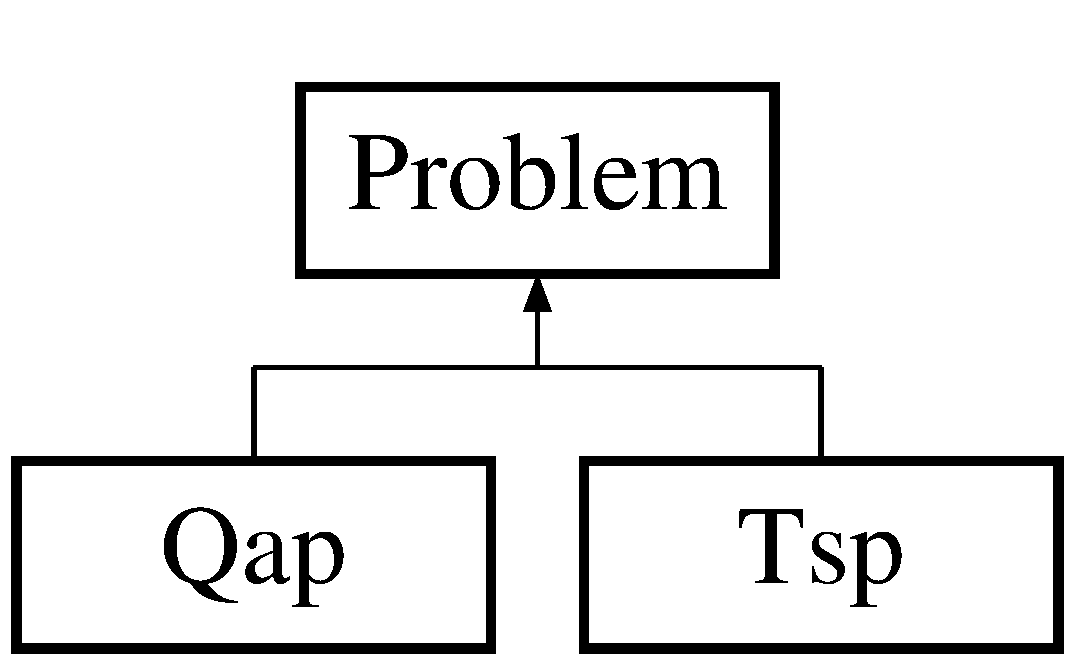
\includegraphics[height=2.000000cm]{class_problem}
\end{center}
\end{figure}
\subsection*{Public Member Functions}
\begin{DoxyCompactItemize}
\item 
\hypertarget{class_problem_a4b9787b3945dbec08e402c0cfd0f646b}{virtual \hyperlink{class_solution}{Solution} $\ast$ \hyperlink{class_problem_a4b9787b3945dbec08e402c0cfd0f646b}{New\+Solution} ()=0}\label{class_problem_a4b9787b3945dbec08e402c0cfd0f646b}

\begin{DoxyCompactList}\small\item\em Método virtual que retorna un puntero del tipo \hyperlink{class_solution}{Solution}, relacionado con la codificación del problema. \end{DoxyCompactList}\item 
\hypertarget{class_problem_adc6176be667576d08cf3e89b65e905f4}{virtual double \hyperlink{class_problem_adc6176be667576d08cf3e89b65e905f4}{Calcular\+Fitness} (\hyperlink{class_solution}{Solution} $\ast$sol)=0}\label{class_problem_adc6176be667576d08cf3e89b65e905f4}

\begin{DoxyCompactList}\small\item\em Método virtual que permite establecer el cálculo del fitness de las soluciones, para cada problema en particular. \end{DoxyCompactList}\item 
\hypertarget{class_problem_ad6a122249b93487f91a64837a056fa75}{virtual double \hyperlink{class_problem_ad6a122249b93487f91a64837a056fa75}{get\+Min\+Values\+Pos} (unsigned int pos)=0}\label{class_problem_ad6a122249b93487f91a64837a056fa75}

\begin{DoxyCompactList}\small\item\em Método virtual que permite retornar el valor para una determinada coordenada, entre los mínimos valores posibles para cada problema en particular. \end{DoxyCompactList}\item 
\hypertarget{class_problem_a2ffe7de8658a25398d6a21dd1b2edfcb}{virtual double \hyperlink{class_problem_a2ffe7de8658a25398d6a21dd1b2edfcb}{get\+Max\+Values\+Pos} (unsigned int pos)=0}\label{class_problem_a2ffe7de8658a25398d6a21dd1b2edfcb}

\begin{DoxyCompactList}\small\item\em Método virtual que permite retornar el valor para una determinada coordenada, entre los maximos valores posibles para cada problema en particular. \end{DoxyCompactList}\item 
\hypertarget{class_problem_a6f72067600654aef0767bce95c4eacdd}{virtual unsigned int \hyperlink{class_problem_a6f72067600654aef0767bce95c4eacdd}{get\+Dimension} ()=0}\label{class_problem_a6f72067600654aef0767bce95c4eacdd}

\begin{DoxyCompactList}\small\item\em Método virtual que permite retornar la dimension en cada problema en particular. \end{DoxyCompactList}\item 
\hypertarget{class_problem_a481dc3e5869cf95b3c539d552e8eeb50}{virtual bool \hyperlink{class_problem_a481dc3e5869cf95b3c539d552e8eeb50}{Es\+Dinamico} ()=0}\label{class_problem_a481dc3e5869cf95b3c539d552e8eeb50}

\begin{DoxyCompactList}\small\item\em Método virtual que permite saber si es dinámico o no un problema en particular. \end{DoxyCompactList}\item 
\hypertarget{class_problem_a0c7025eb5127b1eda7988cceadc00da6}{virtual void \hyperlink{class_problem_a0c7025eb5127b1eda7988cceadc00da6}{step} (std\+::vector$<$ std\+::vector$<$ double $>$ $>$, int)=0}\label{class_problem_a0c7025eb5127b1eda7988cceadc00da6}

\begin{DoxyCompactList}\small\item\em Método virtual que permite realizar cambio en el espacio de búsqueda en un problema en particular que sea dinámico. \end{DoxyCompactList}\item 
\hypertarget{class_problem_a4b9787b3945dbec08e402c0cfd0f646b}{virtual \hyperlink{class_solution}{Solution} $\ast$ \hyperlink{class_problem_a4b9787b3945dbec08e402c0cfd0f646b}{New\+Solution} ()=0}\label{class_problem_a4b9787b3945dbec08e402c0cfd0f646b}

\begin{DoxyCompactList}\small\item\em Método virtual que retorna un puntero del tipo \hyperlink{class_solution}{Solution}, relacionado con la codificación del problema. \end{DoxyCompactList}\item 
\hypertarget{class_problem_adc6176be667576d08cf3e89b65e905f4}{virtual double \hyperlink{class_problem_adc6176be667576d08cf3e89b65e905f4}{Calcular\+Fitness} (\hyperlink{class_solution}{Solution} $\ast$sol)=0}\label{class_problem_adc6176be667576d08cf3e89b65e905f4}

\begin{DoxyCompactList}\small\item\em Método virtual que permite establecer el cálculo del fitness de las soluciones, para cada problema en particular. \end{DoxyCompactList}\item 
\hypertarget{class_problem_ad6a122249b93487f91a64837a056fa75}{virtual double \hyperlink{class_problem_ad6a122249b93487f91a64837a056fa75}{get\+Min\+Values\+Pos} (unsigned int pos)=0}\label{class_problem_ad6a122249b93487f91a64837a056fa75}

\begin{DoxyCompactList}\small\item\em Método virtual que permite retornar el valor para una determinada coordenada, entre los mínimos valores posibles para cada problema en particular. \end{DoxyCompactList}\item 
\hypertarget{class_problem_a2ffe7de8658a25398d6a21dd1b2edfcb}{virtual double \hyperlink{class_problem_a2ffe7de8658a25398d6a21dd1b2edfcb}{get\+Max\+Values\+Pos} (unsigned int pos)=0}\label{class_problem_a2ffe7de8658a25398d6a21dd1b2edfcb}

\begin{DoxyCompactList}\small\item\em Método virtual que permite retornar el valor para una determinada coordenada, entre los maximos valores posibles para cada problema en particular. \end{DoxyCompactList}\item 
\hypertarget{class_problem_a6f72067600654aef0767bce95c4eacdd}{virtual unsigned int \hyperlink{class_problem_a6f72067600654aef0767bce95c4eacdd}{get\+Dimension} ()=0}\label{class_problem_a6f72067600654aef0767bce95c4eacdd}

\begin{DoxyCompactList}\small\item\em Método virtual que permite retornar la dimension en cada problema en particular. \end{DoxyCompactList}\item 
\hypertarget{class_problem_a481dc3e5869cf95b3c539d552e8eeb50}{virtual bool \hyperlink{class_problem_a481dc3e5869cf95b3c539d552e8eeb50}{Es\+Dinamico} ()=0}\label{class_problem_a481dc3e5869cf95b3c539d552e8eeb50}

\begin{DoxyCompactList}\small\item\em Método virtual que permite saber si es dinámico o no un problema en particular. \end{DoxyCompactList}\item 
\hypertarget{class_problem_a0c7025eb5127b1eda7988cceadc00da6}{virtual void \hyperlink{class_problem_a0c7025eb5127b1eda7988cceadc00da6}{step} (std\+::vector$<$ std\+::vector$<$ double $>$ $>$, int)=0}\label{class_problem_a0c7025eb5127b1eda7988cceadc00da6}

\begin{DoxyCompactList}\small\item\em Método virtual que permite realizar cambio en el espacio de búsqueda en un problema en particular que sea dinámico. \end{DoxyCompactList}\end{DoxyCompactItemize}
\subsection*{Static Public Member Functions}
\begin{DoxyCompactItemize}
\item 
static \hyperlink{class_problem}{Problem} $\ast$ \hyperlink{class_problem_a4455f10e5a7e568a4c4359c53e73c547}{instance} ()
\begin{DoxyCompactList}\small\item\em return the pointer to the singleton instance \end{DoxyCompactList}\item 
\hypertarget{class_problem_a8ef29b0090589205c8cd920082e2469b}{static \hyperlink{class_problem}{Problem} $\ast$ \hyperlink{class_problem_a8ef29b0090589205c8cd920082e2469b}{instance} ()}\label{class_problem_a8ef29b0090589205c8cd920082e2469b}

\begin{DoxyCompactList}\small\item\em return the pointer to the singleton instance \end{DoxyCompactList}\end{DoxyCompactItemize}


\subsection{Detailed Description}
Clase abstracta \hyperlink{class_problem}{Problem}. 

\subsection{Member Function Documentation}
\hypertarget{class_problem_a4455f10e5a7e568a4c4359c53e73c547}{\index{Problem@{Problem}!instance@{instance}}
\index{instance@{instance}!Problem@{Problem}}
\subsubsection[{instance}]{\setlength{\rightskip}{0pt plus 5cm}{\bf Problem} $\ast$ Problem\+::instance (
\begin{DoxyParamCaption}
{}
\end{DoxyParamCaption}
)\hspace{0.3cm}{\ttfamily [static]}}}\label{class_problem_a4455f10e5a7e568a4c4359c53e73c547}


return the pointer to the singleton instance 

\begin{DoxyReturn}{Returns}
Retorna puntero del tipo \hyperlink{class_problem}{Problem}, con problema particular para Ackley

Retorna puntero del tipo \hyperlink{class_problem}{Problem}, con problema particular para \hyperlink{class_tsp}{Tsp} 
\end{DoxyReturn}


The documentation for this class was generated from the following files\+:\begin{DoxyCompactItemize}
\item 
Q\+A\+P\+\_\+\+P\+E\+R\+M/problem.\+h\item 
Q\+A\+P\+\_\+\+P\+E\+R\+M/problem.\+cpp\end{DoxyCompactItemize}

\hypertarget{class_qap}{\section{Referencia de la Clase Qap}
\label{class_qap}\index{Qap@{Qap}}
}


Diagrama de herencias de Qap
\nopagebreak
\begin{figure}[H]
\begin{center}
\leavevmode
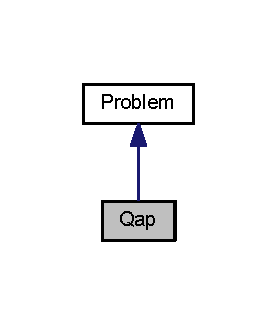
\includegraphics[width=133pt]{class_qap__inherit__graph}
\end{center}
\end{figure}


Diagrama de colaboración para Qap\+:
\nopagebreak
\begin{figure}[H]
\begin{center}
\leavevmode
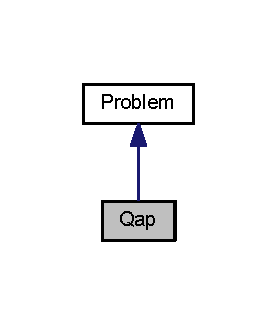
\includegraphics[width=133pt]{class_qap__coll__graph}
\end{center}
\end{figure}
\subsection*{Métodos públicos}
\begin{DoxyCompactItemize}
\item 
\hyperlink{class_solution}{Solution} $\ast$ \hyperlink{class_qap_a4493347601b4458092eb443ee8499743}{New\+Solution} ()
\begin{DoxyCompactList}\small\item\em Redefinicion del método para la clase \hyperlink{class_qap}{Qap}. \end{DoxyCompactList}\item 
double \hyperlink{class_qap_a05d324d41f7d70c8057b7b35a2f2aeab}{Calcular\+Fitness} (\hyperlink{class_solution}{Solution} $\ast$sol)
\begin{DoxyCompactList}\small\item\em Redefinicion del método para la clase \hyperlink{class_qap}{Qap}. \end{DoxyCompactList}\item 
double \hyperlink{class_qap_a8b736df9c6b69a4f1f2c76921b1d9992}{get\+Min\+Values\+Pos} (unsigned int pos)
\begin{DoxyCompactList}\small\item\em Redefinicion del método para la clase \hyperlink{class_qap}{Qap}. \end{DoxyCompactList}\item 
double \hyperlink{class_qap_ac0d42b8ed406cad3c960505628f4f35c}{get\+Max\+Values\+Pos} (unsigned int pos)
\begin{DoxyCompactList}\small\item\em Redefinicion del método para la clase \hyperlink{class_qap}{Qap}. \end{DoxyCompactList}\item 
unsigned int \hyperlink{class_qap_a82bf0c0567c7e5bbfcef5ec7b4281409}{get\+Dimension} ()
\begin{DoxyCompactList}\small\item\em Redefinicion del método para la clase \hyperlink{class_qap}{Qap}. \end{DoxyCompactList}\item 
bool \hyperlink{class_qap_ac338b0a23c2565cd014a193569a33870}{Es\+Dinamico} ()
\begin{DoxyCompactList}\small\item\em Redefinicion del método para la clase \hyperlink{class_qap}{Qap}. \end{DoxyCompactList}\item 
void \hyperlink{class_qap_a3bb1b7cc62a0f0f0ddd9e2644cea2b7f}{step} (std\+::vector$<$ std\+::vector$<$ double $>$ $>$, int)
\begin{DoxyCompactList}\small\item\em Redefinicion del método para la clase \hyperlink{class_qap}{Qap}. \end{DoxyCompactList}\item 
void \hyperlink{class_qap_a0c90fc0c866ba30a979a8a28e7d95336}{read\+Q\+A\+P\+Problem\+File} (string filename)
\end{DoxyCompactItemize}
\subsection*{Otros miembros heredados}


\subsection{Documentación de las funciones miembro}
\hypertarget{class_qap_a05d324d41f7d70c8057b7b35a2f2aeab}{\index{Qap@{Qap}!Calcular\+Fitness@{Calcular\+Fitness}}
\index{Calcular\+Fitness@{Calcular\+Fitness}!Qap@{Qap}}
\subsubsection[{Calcular\+Fitness}]{\setlength{\rightskip}{0pt plus 5cm}double Qap\+::\+Calcular\+Fitness (
\begin{DoxyParamCaption}
\item[{{\bf Solution} $\ast$}]{sol}
\end{DoxyParamCaption}
)\hspace{0.3cm}{\ttfamily [virtual]}}}\label{class_qap_a05d324d41f7d70c8057b7b35a2f2aeab}


Redefinicion del método para la clase \hyperlink{class_qap}{Qap}. 


\begin{DoxyParams}{Parámetros}
{\em sol} & Puntero a la solución, que se desea determinar su fitness en la subclase \hyperlink{class_tsp}{Tsp} \\
\hline
\end{DoxyParams}


Implementa \hyperlink{class_problem_adc6176be667576d08cf3e89b65e905f4}{Problem}.



Gráfico de llamadas para esta función\+:
\nopagebreak
\begin{figure}[H]
\begin{center}
\leavevmode
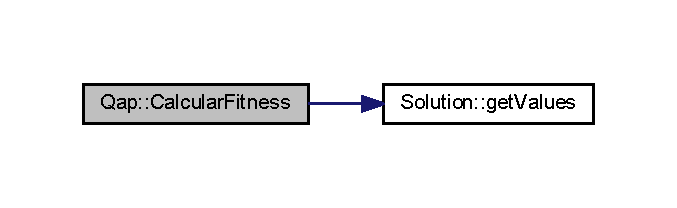
\includegraphics[width=325pt]{class_qap_a05d324d41f7d70c8057b7b35a2f2aeab_cgraph}
\end{center}
\end{figure}


\hypertarget{class_qap_ac338b0a23c2565cd014a193569a33870}{\index{Qap@{Qap}!Es\+Dinamico@{Es\+Dinamico}}
\index{Es\+Dinamico@{Es\+Dinamico}!Qap@{Qap}}
\subsubsection[{Es\+Dinamico}]{\setlength{\rightskip}{0pt plus 5cm}bool Qap\+::\+Es\+Dinamico (
\begin{DoxyParamCaption}
{}
\end{DoxyParamCaption}
)\hspace{0.3cm}{\ttfamily [virtual]}}}\label{class_qap_ac338b0a23c2565cd014a193569a33870}


Redefinicion del método para la clase \hyperlink{class_qap}{Qap}. 

\begin{DoxyReturn}{Devuelve}
Retorna valor del tipo booleano, con la respuesta de si es o no, dinámico el problema 
\end{DoxyReturn}


Implementa \hyperlink{class_problem_a481dc3e5869cf95b3c539d552e8eeb50}{Problem}.

\hypertarget{class_qap_a82bf0c0567c7e5bbfcef5ec7b4281409}{\index{Qap@{Qap}!get\+Dimension@{get\+Dimension}}
\index{get\+Dimension@{get\+Dimension}!Qap@{Qap}}
\subsubsection[{get\+Dimension}]{\setlength{\rightskip}{0pt plus 5cm}unsigned int Qap\+::get\+Dimension (
\begin{DoxyParamCaption}
{}
\end{DoxyParamCaption}
)\hspace{0.3cm}{\ttfamily [virtual]}}}\label{class_qap_a82bf0c0567c7e5bbfcef5ec7b4281409}


Redefinicion del método para la clase \hyperlink{class_qap}{Qap}. 

\begin{DoxyReturn}{Devuelve}
Retorna valor del tipo entero sin signo, con el valor de la dimensión del problema 
\end{DoxyReturn}


Implementa \hyperlink{class_problem_a6f72067600654aef0767bce95c4eacdd}{Problem}.

\hypertarget{class_qap_ac0d42b8ed406cad3c960505628f4f35c}{\index{Qap@{Qap}!get\+Max\+Values\+Pos@{get\+Max\+Values\+Pos}}
\index{get\+Max\+Values\+Pos@{get\+Max\+Values\+Pos}!Qap@{Qap}}
\subsubsection[{get\+Max\+Values\+Pos}]{\setlength{\rightskip}{0pt plus 5cm}double Qap\+::get\+Max\+Values\+Pos (
\begin{DoxyParamCaption}
\item[{unsigned int}]{pos}
\end{DoxyParamCaption}
)\hspace{0.3cm}{\ttfamily [virtual]}}}\label{class_qap_ac0d42b8ed406cad3c960505628f4f35c}


Redefinicion del método para la clase \hyperlink{class_qap}{Qap}. 


\begin{DoxyParams}{Parámetros}
{\em pos} & Posición de la coordenada\\
\hline
\end{DoxyParams}
\begin{DoxyReturn}{Devuelve}
Retorna valor del tipo double, con el valor de esa coordenada para los máximos valores 
\end{DoxyReturn}


Implementa \hyperlink{class_problem_a2ffe7de8658a25398d6a21dd1b2edfcb}{Problem}.

\hypertarget{class_qap_a8b736df9c6b69a4f1f2c76921b1d9992}{\index{Qap@{Qap}!get\+Min\+Values\+Pos@{get\+Min\+Values\+Pos}}
\index{get\+Min\+Values\+Pos@{get\+Min\+Values\+Pos}!Qap@{Qap}}
\subsubsection[{get\+Min\+Values\+Pos}]{\setlength{\rightskip}{0pt plus 5cm}double Qap\+::get\+Min\+Values\+Pos (
\begin{DoxyParamCaption}
\item[{unsigned int}]{pos}
\end{DoxyParamCaption}
)\hspace{0.3cm}{\ttfamily [virtual]}}}\label{class_qap_a8b736df9c6b69a4f1f2c76921b1d9992}


Redefinicion del método para la clase \hyperlink{class_qap}{Qap}. 


\begin{DoxyParams}{Parámetros}
{\em pos} & Indica la posición de la coordenada\\
\hline
\end{DoxyParams}
\begin{DoxyReturn}{Devuelve}
Retorna valor del tipo double, con el valor de esa coordenada para los mínimos valores 
\end{DoxyReturn}


Implementa \hyperlink{class_problem_ad6a122249b93487f91a64837a056fa75}{Problem}.

\hypertarget{class_qap_a4493347601b4458092eb443ee8499743}{\index{Qap@{Qap}!New\+Solution@{New\+Solution}}
\index{New\+Solution@{New\+Solution}!Qap@{Qap}}
\subsubsection[{New\+Solution}]{\setlength{\rightskip}{0pt plus 5cm}{\bf Solution} $\ast$ Qap\+::\+New\+Solution (
\begin{DoxyParamCaption}
{}
\end{DoxyParamCaption}
)\hspace{0.3cm}{\ttfamily [virtual]}}}\label{class_qap_a4493347601b4458092eb443ee8499743}


Redefinicion del método para la clase \hyperlink{class_qap}{Qap}. 

\begin{DoxyReturn}{Devuelve}
Retorna puntero del tipo \hyperlink{class_solution}{Solution}, con una nueva solución relacionada con la codificación en particular para el problema, específicamente Solution\+R\+N 
\end{DoxyReturn}


Implementa \hyperlink{class_problem_a4b9787b3945dbec08e402c0cfd0f646b}{Problem}.

\hypertarget{class_qap_a0c90fc0c866ba30a979a8a28e7d95336}{\index{Qap@{Qap}!read\+Q\+A\+P\+Problem\+File@{read\+Q\+A\+P\+Problem\+File}}
\index{read\+Q\+A\+P\+Problem\+File@{read\+Q\+A\+P\+Problem\+File}!Qap@{Qap}}
\subsubsection[{read\+Q\+A\+P\+Problem\+File}]{\setlength{\rightskip}{0pt plus 5cm}void Qap\+::read\+Q\+A\+P\+Problem\+File (
\begin{DoxyParamCaption}
\item[{string}]{filename}
\end{DoxyParamCaption}
)}}\label{class_qap_a0c90fc0c866ba30a979a8a28e7d95336}
int k = 1; \hypertarget{class_qap_a3bb1b7cc62a0f0f0ddd9e2644cea2b7f}{\index{Qap@{Qap}!step@{step}}
\index{step@{step}!Qap@{Qap}}
\subsubsection[{step}]{\setlength{\rightskip}{0pt plus 5cm}void Qap\+::step (
\begin{DoxyParamCaption}
\item[{std\+::vector$<$ std\+::vector$<$ double $>$ $>$}]{, }
\item[{int}]{}
\end{DoxyParamCaption}
)\hspace{0.3cm}{\ttfamily [virtual]}}}\label{class_qap_a3bb1b7cc62a0f0f0ddd9e2644cea2b7f}


Redefinicion del método para la clase \hyperlink{class_qap}{Qap}. 


\begin{DoxyParams}{Parámetros}
{\em datos} & Arreglo de arreglo con valores de todas las plantas presentes en el patio \\
\hline
{\em iter} & Numero de la iteracion actual \\
\hline
\end{DoxyParams}


Implementa \hyperlink{class_problem_a0c7025eb5127b1eda7988cceadc00da6}{Problem}.



La documentación para esta clase fue generada a partir de los siguientes ficheros\+:\begin{DoxyCompactItemize}
\item 
Q\+A\+P\+\_\+\+P\+E\+R\+M/Qap.\+h\item 
Q\+A\+P\+\_\+\+P\+E\+R\+M/Qap.\+cpp\end{DoxyCompactItemize}

\hypertarget{classrand31dc}{\section{Referencia de la Clase rand31dc}
\label{classrand31dc}\index{rand31dc@{rand31dc}}
}


31 bit pseudo-\/random number generator based on Lehmer (1951); Lewis, Goodman \& Miller (1969); Park \& Miller (1983)  




{\ttfamily \#include $<$rand31pmc.\+h$>$}

\subsection*{Métodos públicos}
\begin{DoxyCompactItemize}
\item 
\hypertarget{classrand31dc_ab57e4bf816dd2d20c052fd951338d845}{\hyperlink{classrand31dc_ab57e4bf816dd2d20c052fd951338d845}{rand31dc} ()}\label{classrand31dc_ab57e4bf816dd2d20c052fd951338d845}

\begin{DoxyCompactList}\small\item\em Constructor sets seed31 to 1, in case no seedi operation is used. \end{DoxyCompactList}\item 
\hypertarget{classrand31dc_a8890a8223643fff52fff7a332e2053c6}{void \hyperlink{classrand31dc_a8890a8223643fff52fff7a332e2053c6}{seedi} (long unsigned int)}\label{classrand31dc_a8890a8223643fff52fff7a332e2053c6}

\begin{DoxyCompactList}\small\item\em Set the seed from a long unsigned integer. If zero is used, then the seed will be set to 1. \end{DoxyCompactList}\item 
\hypertarget{classrand31dc_a6694db8a614a793f4a00473f8b7ea409}{long unsigned int \hyperlink{classrand31dc_a6694db8a614a793f4a00473f8b7ea409}{ranlui} (void)}\label{classrand31dc_a6694db8a614a793f4a00473f8b7ea409}

\begin{DoxyCompactList}\small\item\em Return next pseudo-\/random value as a long unsigned integer. \end{DoxyCompactList}\item 
\hypertarget{classrand31dc_ae3fd0aa4320143ee001e408587bb7844}{float \hyperlink{classrand31dc_ae3fd0aa4320143ee001e408587bb7844}{ranf} (void)}\label{classrand31dc_ae3fd0aa4320143ee001e408587bb7844}

\begin{DoxyCompactList}\small\item\em Return next pseudo-\/random value as a floating point value. \end{DoxyCompactList}\end{DoxyCompactItemize}


\subsection{Descripción detallada}
31 bit pseudo-\/random number generator based on Lehmer (1951); Lewis, Goodman \& Miller (1969); Park \& Miller (1983) 

La documentación para esta clase fue generada a partir de los siguientes ficheros\+:\begin{DoxyCompactItemize}
\item 
B\+A\+S\+E/rand31pmc.\+h\item 
B\+A\+S\+E/rand31pmc.\+cpp\end{DoxyCompactItemize}

\hypertarget{class_solution}{\section{Solution Class Reference}
\label{class_solution}\index{Solution@{Solution}}
}


Clase Abstracta \hyperlink{class_solution}{Solution}.  


Inheritance diagram for Solution\+:\begin{figure}[H]
\begin{center}
\leavevmode
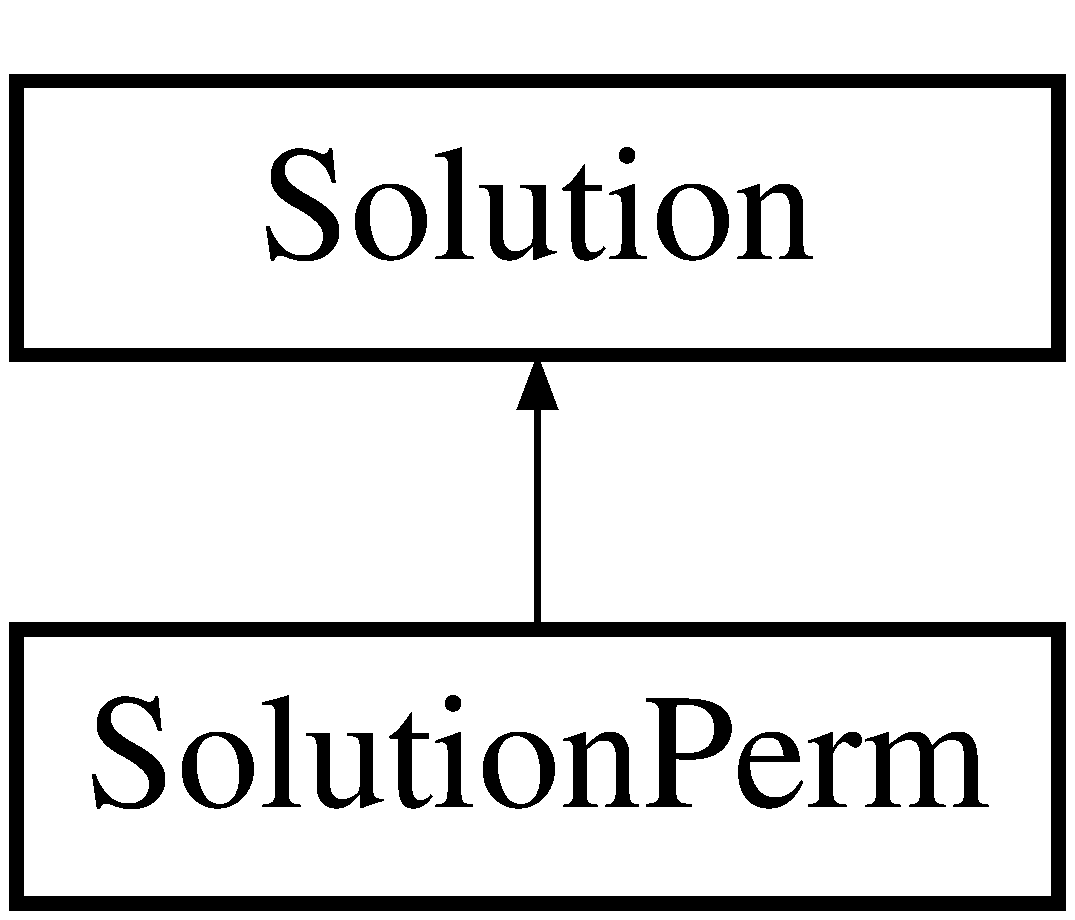
\includegraphics[height=2.000000cm]{class_solution}
\end{center}
\end{figure}
\subsection*{Public Member Functions}
\begin{DoxyCompactItemize}
\item 
\hypertarget{class_solution_ab55bd4b023d596ce11aaf737b9a6123b}{\hyperlink{class_solution_ab55bd4b023d596ce11aaf737b9a6123b}{Solution} ()}\label{class_solution_ab55bd4b023d596ce11aaf737b9a6123b}

\begin{DoxyCompactList}\small\item\em Constructor por defecto de la clase. \end{DoxyCompactList}\item 
\hypertarget{class_solution_a5d245f7409aacf6ace5e965b7879a580}{\hyperlink{class_solution_a5d245f7409aacf6ace5e965b7879a580}{$\sim$\+Solution} ()}\label{class_solution_a5d245f7409aacf6ace5e965b7879a580}

\begin{DoxyCompactList}\small\item\em Destructor de la clase. \end{DoxyCompactList}\item 
void \hyperlink{class_solution_a14efa947803fd35d6af01aaf83eed17b}{set\+Fitness} (double \+\_\+fitness)
\begin{DoxyCompactList}\small\item\em Establece el fitness de la solucion. \end{DoxyCompactList}\item 
double \hyperlink{class_solution_a794776f952a06bb4a4a7e0f198efcfa2}{get\+Fitness} ()
\begin{DoxyCompactList}\small\item\em Retorna el fitness de la solucion. \end{DoxyCompactList}\item 
unsigned int \hyperlink{class_solution_aeb1c4eb1bd5aca251f43c92720c36d25}{get\+Dimension} ()
\begin{DoxyCompactList}\small\item\em Retorna la dimension de la Solucion. \end{DoxyCompactList}\item 
\hypertarget{class_solution_a856741c28b047bae68aa7cb3721d30bb}{virtual void $\ast$ \hyperlink{class_solution_a856741c28b047bae68aa7cb3721d30bb}{get\+Values} ()=0}\label{class_solution_a856741c28b047bae68aa7cb3721d30bb}

\begin{DoxyCompactList}\small\item\em Retorna el valores particulares de las soluciones. \end{DoxyCompactList}\item 
\hypertarget{class_solution_aa66480352ac71f9366df6b409f99dedf}{virtual double \hyperlink{class_solution_aa66480352ac71f9366df6b409f99dedf}{Distance} (\hyperlink{class_solution}{Solution} $\ast$other\+\_\+sol)=0}\label{class_solution_aa66480352ac71f9366df6b409f99dedf}

\begin{DoxyCompactList}\small\item\em Retorna la distancia entre las soluciones. \end{DoxyCompactList}\item 
\hypertarget{class_solution_a232b4bd1064e9bae8ff4c0cbe82f6be6}{virtual \hyperlink{class_solution}{Solution} $\ast$ \hyperlink{class_solution_a232b4bd1064e9bae8ff4c0cbe82f6be6}{Extend\+Solution} (double X\+\_\+i)=0}\label{class_solution_a232b4bd1064e9bae8ff4c0cbe82f6be6}

\begin{DoxyCompactList}\small\item\em Para los valores de la solucion actual, se modifican (extienden) retornando otra nueva solucion. \end{DoxyCompactList}\item 
\hypertarget{class_solution_a57453daeb5427edff95ae110a5f6ae9b}{virtual void \hyperlink{class_solution_a57453daeb5427edff95ae110a5f6ae9b}{show\+\_\+solution} (ofstream \&out\+\_\+distill)=0}\label{class_solution_a57453daeb5427edff95ae110a5f6ae9b}

\begin{DoxyCompactList}\small\item\em Registra las componentes de la solucion y su fitness en un archivo. \end{DoxyCompactList}\end{DoxyCompactItemize}
\subsection*{Protected Attributes}
\begin{DoxyCompactItemize}
\item 
\hypertarget{class_solution_a215acc6c80b2c16071246b9ded8f32ab}{double \hyperlink{class_solution_a215acc6c80b2c16071246b9ded8f32ab}{fitness}}\label{class_solution_a215acc6c80b2c16071246b9ded8f32ab}

\begin{DoxyCompactList}\small\item\em Fitness de la solucion. \end{DoxyCompactList}\item 
\hypertarget{class_solution_a7111f2ad10bd9e1696d3e19c1b5bff09}{unsigned int \hyperlink{class_solution_a7111f2ad10bd9e1696d3e19c1b5bff09}{dimension}}\label{class_solution_a7111f2ad10bd9e1696d3e19c1b5bff09}

\begin{DoxyCompactList}\small\item\em Dimension de la solucion. \end{DoxyCompactList}\end{DoxyCompactItemize}


\subsection{Detailed Description}
Clase Abstracta \hyperlink{class_solution}{Solution}. 

En esta clase, se define la estructura general de las distintas soluciones a ser codificadas.

Al ser una clase general, los métodos más particulares y específicos que se requieran para cada una de las distintas codificaciones, se definen como {\bfseries virtuales}. En todas las subclases de \hyperlink{class_solution}{Solution}, obligatoriamente se deben redefinir esos métodos. Los cuales son\+:


\begin{DoxyItemize}
\item get\+Values 
\item Distance 
\item Extend\+Solution 
\item show\+\_\+solution 
\end{DoxyItemize}

De los cuales se comenta más abajo. 

\subsection{Member Function Documentation}
\hypertarget{class_solution_aeb1c4eb1bd5aca251f43c92720c36d25}{\index{Solution@{Solution}!get\+Dimension@{get\+Dimension}}
\index{get\+Dimension@{get\+Dimension}!Solution@{Solution}}
\subsubsection[{get\+Dimension}]{\setlength{\rightskip}{0pt plus 5cm}unsigned int Solution\+::get\+Dimension (
\begin{DoxyParamCaption}
{}
\end{DoxyParamCaption}
)}}\label{class_solution_aeb1c4eb1bd5aca251f43c92720c36d25}


Retorna la dimension de la Solucion. 

\begin{DoxyReturn}{Returns}
Retorna la dimension de la solucion 
\end{DoxyReturn}
\hypertarget{class_solution_a794776f952a06bb4a4a7e0f198efcfa2}{\index{Solution@{Solution}!get\+Fitness@{get\+Fitness}}
\index{get\+Fitness@{get\+Fitness}!Solution@{Solution}}
\subsubsection[{get\+Fitness}]{\setlength{\rightskip}{0pt plus 5cm}double Solution\+::get\+Fitness (
\begin{DoxyParamCaption}
{}
\end{DoxyParamCaption}
)}}\label{class_solution_a794776f952a06bb4a4a7e0f198efcfa2}


Retorna el fitness de la solucion. 

\begin{DoxyReturn}{Returns}
Retorna el fitness de la solucion 
\end{DoxyReturn}
\hypertarget{class_solution_a14efa947803fd35d6af01aaf83eed17b}{\index{Solution@{Solution}!set\+Fitness@{set\+Fitness}}
\index{set\+Fitness@{set\+Fitness}!Solution@{Solution}}
\subsubsection[{set\+Fitness}]{\setlength{\rightskip}{0pt plus 5cm}void Solution\+::set\+Fitness (
\begin{DoxyParamCaption}
\item[{double}]{\+\_\+fitness}
\end{DoxyParamCaption}
)}}\label{class_solution_a14efa947803fd35d6af01aaf83eed17b}


Establece el fitness de la solucion. 


\begin{DoxyParams}{Parameters}
{\em \+\_\+fitness} & valor a establecer como fitness de la solucion \\
\hline
\end{DoxyParams}


The documentation for this class was generated from the following files\+:\begin{DoxyCompactItemize}
\item 
B\+A\+S\+E/solution.\+h\item 
B\+A\+S\+E/solution.\+cpp\end{DoxyCompactItemize}

\hypertarget{class_solution_perm}{\section{Referencia de la Clase Solution\+Perm}
\label{class_solution_perm}\index{Solution\+Perm@{Solution\+Perm}}
}
Diagrama de herencias de Solution\+Perm\begin{figure}[H]
\begin{center}
\leavevmode
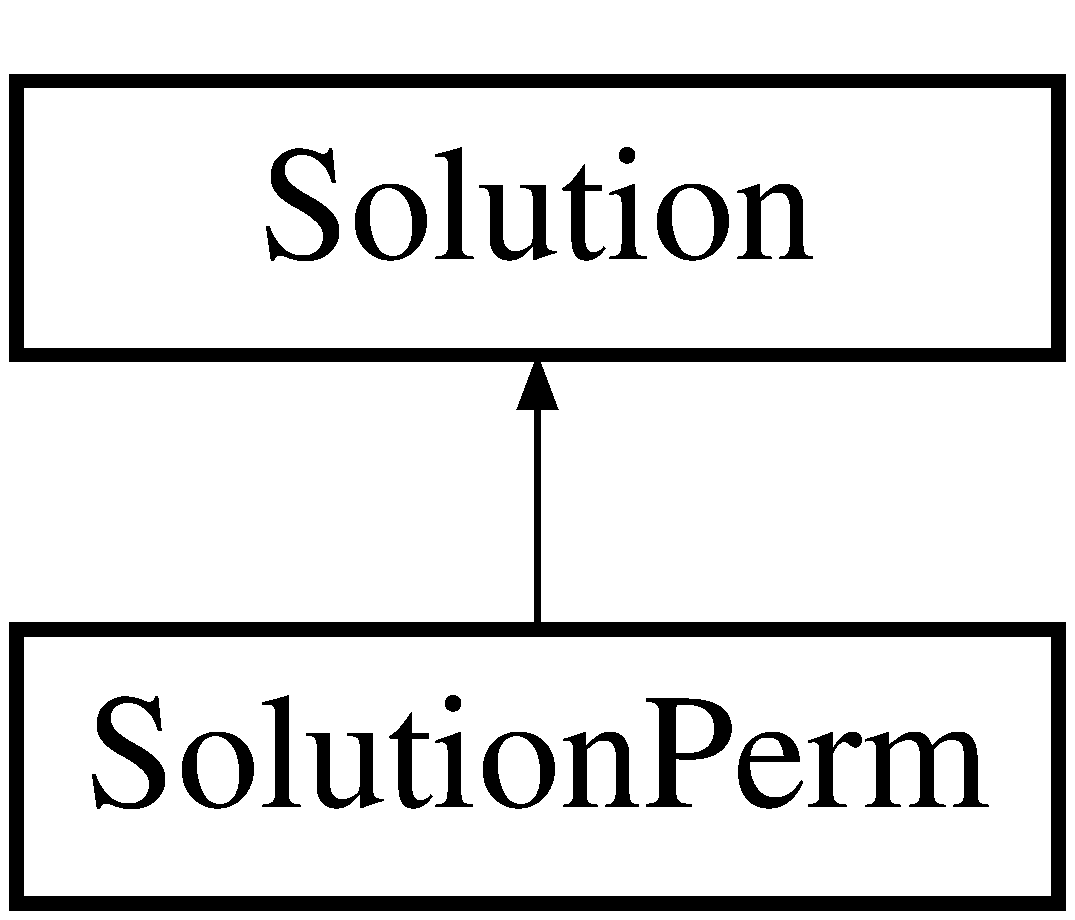
\includegraphics[height=2.000000cm]{class_solution_perm}
\end{center}
\end{figure}
\subsection*{Métodos públicos}
\begin{DoxyCompactItemize}
\item 
\hypertarget{class_solution_perm_a71ea7ad7c43c4b9ce6058640acd24bae}{{\bfseries Solution\+Perm} (vector$<$ int $>$ \+\_\+values)}\label{class_solution_perm_a71ea7ad7c43c4b9ce6058640acd24bae}

\item 
\hypertarget{class_solution_perm_a19e9bfc6873053fa4cb2644fb0ceadba}{double \hyperlink{class_solution_perm_a19e9bfc6873053fa4cb2644fb0ceadba}{Delta} (double d, double X\+\_\+i)}\label{class_solution_perm_a19e9bfc6873053fa4cb2644fb0ceadba}

\begin{DoxyCompactList}\small\item\em Definicion de la distancia a desplazar a la planta hija. \end{DoxyCompactList}\item 
\hypertarget{class_solution_perm_a087dca9092baa1bfe8d52270f3e927a5}{void $\ast$ \hyperlink{class_solution_perm_a087dca9092baa1bfe8d52270f3e927a5}{get\+Values} ()}\label{class_solution_perm_a087dca9092baa1bfe8d52270f3e927a5}

\begin{DoxyCompactList}\small\item\em Redefinicion metodo virtual\+: retorna valores propios de la solucion. \end{DoxyCompactList}\item 
\hypertarget{class_solution_perm_a8cdccc3689d67ddb773a5384bb0be7f1}{double \hyperlink{class_solution_perm_a8cdccc3689d67ddb773a5384bb0be7f1}{Distance} (\hyperlink{class_solution}{Solution} $\ast$other\+\_\+sol)}\label{class_solution_perm_a8cdccc3689d67ddb773a5384bb0be7f1}

\begin{DoxyCompactList}\small\item\em Redefinicion metodo virtual\+: retorna la distancia euclidiana entre las soluciones. \end{DoxyCompactList}\item 
\hypertarget{class_solution_perm_aef2c6326c6a9d77b0e33ed9c024dc2e1}{double {\bfseries Distance} (vector$<$ int $>$ perm, vector$<$ int $>$ perm\+\_\+prima)}\label{class_solution_perm_aef2c6326c6a9d77b0e33ed9c024dc2e1}

\item 
\hypertarget{class_solution_perm_ae2d233dbbd83af831e7fe0fde16906ff}{\hyperlink{class_solution}{Solution} $\ast$ \hyperlink{class_solution_perm_ae2d233dbbd83af831e7fe0fde16906ff}{Extend\+Solution} (double X\+\_\+i)}\label{class_solution_perm_ae2d233dbbd83af831e7fe0fde16906ff}

\begin{DoxyCompactList}\small\item\em Redefinicion metodo virtual\+: retorna solucion extendida. \end{DoxyCompactList}\item 
void \hyperlink{class_solution_perm_a4ac02ebe89d0c95ed85effdf86849eef}{show\+\_\+solution} (ofstream \&out\+\_\+distill)
\begin{DoxyCompactList}\small\item\em Redefinicion metodo virtual\+: desplegar las componentes de la solucion. \end{DoxyCompactList}\item 
vector$<$ int $>$ \hyperlink{class_solution_perm_a0ccb4febe47f43f0f853ee457e43836f}{generate\+Permutation} (int size)
\end{DoxyCompactItemize}
\subsection*{Otros miembros heredados}


\subsection{Documentación de las funciones miembro}
\hypertarget{class_solution_perm_a0ccb4febe47f43f0f853ee457e43836f}{\index{Solution\+Perm@{Solution\+Perm}!generate\+Permutation@{generate\+Permutation}}
\index{generate\+Permutation@{generate\+Permutation}!Solution\+Perm@{Solution\+Perm}}
\subsubsection[{generate\+Permutation}]{\setlength{\rightskip}{0pt plus 5cm}vector$<$ int $>$ Solution\+Perm\+::generate\+Permutation (
\begin{DoxyParamCaption}
\item[{int}]{size}
\end{DoxyParamCaption}
)}}\label{class_solution_perm_a0ccb4febe47f43f0f853ee457e43836f}
\begin{DoxyReturn}{Devuelve}
permutation generated as a integer vector 
\end{DoxyReturn}

\begin{DoxyParams}{Parámetros}
{\em size} & number of elements \\
\hline
\end{DoxyParams}
\hypertarget{class_solution_perm_a4ac02ebe89d0c95ed85effdf86849eef}{\index{Solution\+Perm@{Solution\+Perm}!show\+\_\+solution@{show\+\_\+solution}}
\index{show\+\_\+solution@{show\+\_\+solution}!Solution\+Perm@{Solution\+Perm}}
\subsubsection[{show\+\_\+solution}]{\setlength{\rightskip}{0pt plus 5cm}void Solution\+Perm\+::show\+\_\+solution (
\begin{DoxyParamCaption}
\item[{ofstream \&}]{out\+\_\+distill}
\end{DoxyParamCaption}
)\hspace{0.3cm}{\ttfamily [virtual]}}}\label{class_solution_perm_a4ac02ebe89d0c95ed85effdf86849eef}


Redefinicion metodo virtual\+: desplegar las componentes de la solucion. 


\begin{DoxyParams}{Parámetros}
{\em out\+\_\+distill} & Nombre del archivo que se agregarán los datos más relevantes del objeto de tipo \hyperlink{class_solution}{Solution}, tales como\+: las coordenadas de éste y su fitness \\
\hline
\end{DoxyParams}


Implementa \hyperlink{class_solution_a57453daeb5427edff95ae110a5f6ae9b}{Solution}.



La documentación para esta clase fue generada a partir de los siguientes ficheros\+:\begin{DoxyCompactItemize}
\item 
B\+A\+S\+E/Solution\+Perm.\+h\item 
B\+A\+S\+E/Solution\+Perm.\+cpp\end{DoxyCompactItemize}

\hypertarget{classtoolbox}{\section{Referencia de la Clase toolbox}
\label{classtoolbox}\index{toolbox@{toolbox}}
}


singleton class (only one object is instantiated) that provides general-\/use methods  




{\ttfamily \#include $<$toolbox.\+h$>$}

\subsection*{Métodos públicos}
\begin{DoxyCompactItemize}
\item 
\hypertarget{classtoolbox_aeccc47e3554b49d0077cd6a1967bf8e8}{void {\bfseries read\+\_\+min\+\_\+values} (string filename)}\label{classtoolbox_aeccc47e3554b49d0077cd6a1967bf8e8}

\item 
\hypertarget{classtoolbox_a70936376f353e24a4a9c98d77d8618b5}{void {\bfseries read\+\_\+max\+\_\+values} (string filename)}\label{classtoolbox_a70936376f353e24a4a9c98d77d8618b5}

\item 
\hypertarget{classtoolbox_ae211afebb8cbf64ad2782cfed4cf80dc}{vector$<$ double $>$ {\bfseries get\+\_\+min\+\_\+values} ()}\label{classtoolbox_ae211afebb8cbf64ad2782cfed4cf80dc}

\item 
\hypertarget{classtoolbox_a00d9224a5611a483523740ff63c88775}{vector$<$ double $>$ {\bfseries get\+\_\+max\+\_\+values} ()}\label{classtoolbox_a00d9224a5611a483523740ff63c88775}

\item 
\hypertarget{classtoolbox_ab447abb1ad0631aa7f9165e447d4b1db}{void \hyperlink{classtoolbox_ab447abb1ad0631aa7f9165e447d4b1db}{sandhill\+\_\+create} (string filename)}\label{classtoolbox_ab447abb1ad0631aa7f9165e447d4b1db}

\begin{DoxyCompactList}\small\item\em create from file \end{DoxyCompactList}\item 
\hypertarget{classtoolbox_a153ecab8241cbbb42d32931d580191c4}{double {\bfseries sandhill\+\_\+fitness} (double x, double y)}\label{classtoolbox_a153ecab8241cbbb42d32931d580191c4}

\item 
\hypertarget{classtoolbox_a29b20e4b3351d1c98a4131cac99778f9}{void {\bfseries sandhill\+\_\+show} ()}\label{classtoolbox_a29b20e4b3351d1c98a4131cac99778f9}

\item 
\hypertarget{classtoolbox_ab63881e5e61501fa7f84414f6612ee05}{void \hyperlink{classtoolbox_ab63881e5e61501fa7f84414f6612ee05}{hold} ()}\label{classtoolbox_ab63881e5e61501fa7f84414f6612ee05}

\begin{DoxyCompactList}\small\item\em stops the execution waiting for an E\+N\+T\+E\+R \end{DoxyCompactList}\item 
\hypertarget{classtoolbox_a0ee32c4d293b8952a4767e2565a0dc38}{void \hyperlink{classtoolbox_a0ee32c4d293b8952a4767e2565a0dc38}{clockstart} ()}\label{classtoolbox_a0ee32c4d293b8952a4767e2565a0dc38}

\begin{DoxyCompactList}\small\item\em start chronometer (counts microseconds until \hyperlink{classtoolbox_a8fe27f13cb254a568c8ec0295e5a734f}{clockstop()} is called) \end{DoxyCompactList}\item 
double \hyperlink{classtoolbox_a8fe27f13cb254a568c8ec0295e5a734f}{clockstop} ()
\begin{DoxyCompactList}\small\item\em stop chronometer \end{DoxyCompactList}\item 
void \hyperlink{classtoolbox_a4ea98edf9956998c061850754a37281d}{seed} (long unsigned int semilla)
\item 
double \hyperlink{classtoolbox_a7b24111985e7dcac53f092e954e0cc07}{azar} ()
\item 
int \hyperlink{classtoolbox_ada9e591755dfbbf32979bc1d3f2f81c6}{azar\+Int} (int n)
\item 
double \hyperlink{classtoolbox_a67450c1434f5b2f278c37b6f78f6c91d}{normal} ()
\begin{DoxyCompactList}\small\item\em as seen in \href{http://www.bearcave.com/misl/misl_tech/wavelets/hurst/random.html}{\tt http\+://www.\+bearcave.\+com/misl/misl\+\_\+tech/wavelets/hurst/random.\+html} \end{DoxyCompactList}\item 
double \hyperlink{classtoolbox_a30631661b56eb3e11b40c118241ba6f6}{normal} (double mu, double sigma)
\item 
double \hyperlink{classtoolbox_a76420d97756e45135baa61e037e03d20}{triangular} (double mode, double min, double max)
\begin{DoxyCompactList}\small\item\em as seen in \href{http://www.brighton-webs.co.uk/distributions/triangular.asp}{\tt http\+://www.\+brighton-\/webs.\+co.\+uk/distributions/triangular.\+asp} \end{DoxyCompactList}\item 
double \hyperlink{classtoolbox_a0daf970243cd9158552300762de3f801}{mod} (double a)
\item 
double \hyperlink{classtoolbox_a1347524ce4a6b1db516421f1c2905e44}{string2double} (string s)
\item 
int \hyperlink{classtoolbox_a86769fb57c8a0b58b14a9946a0c90043}{string2int} (string s)
\item 
string \hyperlink{classtoolbox_afb97b8bab923a8c293ff5aa944ed64f7}{double2string} (double d, int prec)
\item 
string \hyperlink{classtoolbox_a4b2268cb178f0ae934f46efffda0450b}{int2string} (int i)
\item 
void \hyperlink{classtoolbox_a2b7ddff386b9bc1f790627f632fae50c}{readparamfile} (string filename)
\item 
void \hyperlink{classtoolbox_a05d6f98094e98e263806b9c7b51fac51}{store\+Variable} (string name, double val, int prec)
\item 
void \hyperlink{classtoolbox_a8f04e33d10ffe547856ded0caf3d5640}{store\+Variable} (string name, string val)
\item 
void \hyperlink{classtoolbox_a53685118cae82122f3a0d083185804b3}{store\+Variable} (string name, int val)
\item 
double \hyperlink{classtoolbox_aa6cb1dff126daa9c34d6e2435143b372}{pval\+\_\+double} (string pname)
\item 
int \hyperlink{classtoolbox_a30135dd53233f8ed0cd68532f51cb002}{pval\+\_\+int} (string pname)
\item 
string \hyperlink{classtoolbox_ad3c9eb0127e47a8ce04922646ade51fc}{pval\+\_\+string} (string pname)
\item 
string \hyperlink{classtoolbox_a67d5356e65a3e93b179f0e48f98cf41c}{filename\+From\+Path} (string path)
\end{DoxyCompactItemize}
\subsection*{Métodos públicos estáticos}
\begin{DoxyCompactItemize}
\item 
\hypertarget{classtoolbox_a3058e36ea4c84178eaa21321a5733cc8}{static \hyperlink{classtoolbox}{toolbox} $\ast$ \hyperlink{classtoolbox_a3058e36ea4c84178eaa21321a5733cc8}{instance} ()}\label{classtoolbox_a3058e36ea4c84178eaa21321a5733cc8}

\begin{DoxyCompactList}\small\item\em return the pointer to the singleton instance \end{DoxyCompactList}\end{DoxyCompactItemize}
\subsection*{Métodos protegidos}
\begin{DoxyCompactItemize}
\item 
\hypertarget{classtoolbox_ae52c33dc9f80c6ce0208a70abde2418e}{\hyperlink{classtoolbox_ae52c33dc9f80c6ce0208a70abde2418e}{toolbox} ()}\label{classtoolbox_ae52c33dc9f80c6ce0208a70abde2418e}

\begin{DoxyCompactList}\small\item\em constructor \end{DoxyCompactList}\item 
\hypertarget{classtoolbox_a384cba887600d141b5c19ada2448522e}{{\bfseries toolbox} (const \hyperlink{classtoolbox}{toolbox} \&)}\label{classtoolbox_a384cba887600d141b5c19ada2448522e}

\item 
\hypertarget{classtoolbox_a22f47dcb9fdf470e56c16c3851a58f7a}{\hyperlink{classtoolbox}{toolbox} \& {\bfseries operator=} (const \hyperlink{classtoolbox}{toolbox} \&)}\label{classtoolbox_a22f47dcb9fdf470e56c16c3851a58f7a}

\end{DoxyCompactItemize}


\subsection{Descripción detallada}
singleton class (only one object is instantiated) that provides general-\/use methods 

\subsection{Documentación de las funciones miembro}
\hypertarget{classtoolbox_a7b24111985e7dcac53f092e954e0cc07}{\index{toolbox@{toolbox}!azar@{azar}}
\index{azar@{azar}!toolbox@{toolbox}}
\subsubsection[{azar}]{\setlength{\rightskip}{0pt plus 5cm}double toolbox\+::azar (
\begin{DoxyParamCaption}
{}
\end{DoxyParamCaption}
)\hspace{0.3cm}{\ttfamily [inline]}}}\label{classtoolbox_a7b24111985e7dcac53f092e954e0cc07}
\begin{DoxyReturn}{Devuelve}
a random number in \mbox{[}0,1) 
\end{DoxyReturn}
\hypertarget{classtoolbox_ada9e591755dfbbf32979bc1d3f2f81c6}{\index{toolbox@{toolbox}!azar\+Int@{azar\+Int}}
\index{azar\+Int@{azar\+Int}!toolbox@{toolbox}}
\subsubsection[{azar\+Int}]{\setlength{\rightskip}{0pt plus 5cm}int toolbox\+::azar\+Int (
\begin{DoxyParamCaption}
\item[{int}]{n}
\end{DoxyParamCaption}
)}}\label{classtoolbox_ada9e591755dfbbf32979bc1d3f2f81c6}
\begin{DoxyReturn}{Devuelve}
a random integer between \mbox{[}0,n-\/1) 
\end{DoxyReturn}
\hypertarget{classtoolbox_a8fe27f13cb254a568c8ec0295e5a734f}{\index{toolbox@{toolbox}!clockstop@{clockstop}}
\index{clockstop@{clockstop}!toolbox@{toolbox}}
\subsubsection[{clockstop}]{\setlength{\rightskip}{0pt plus 5cm}double toolbox\+::clockstop (
\begin{DoxyParamCaption}
{}
\end{DoxyParamCaption}
)}}\label{classtoolbox_a8fe27f13cb254a568c8ec0295e5a734f}


stop chronometer 

\begin{DoxyReturn}{Devuelve}
elapsed time in microseconds since \hyperlink{classtoolbox_a0ee32c4d293b8952a4767e2565a0dc38}{clockstart()} was called 
\end{DoxyReturn}
\hypertarget{classtoolbox_afb97b8bab923a8c293ff5aa944ed64f7}{\index{toolbox@{toolbox}!double2string@{double2string}}
\index{double2string@{double2string}!toolbox@{toolbox}}
\subsubsection[{double2string}]{\setlength{\rightskip}{0pt plus 5cm}string toolbox\+::double2string (
\begin{DoxyParamCaption}
\item[{double}]{d, }
\item[{int}]{prec}
\end{DoxyParamCaption}
)}}\label{classtoolbox_afb97b8bab923a8c293ff5aa944ed64f7}
\begin{DoxyReturn}{Devuelve}
string from double (warning\+: doesn't check that the input can be 'translated') 
\end{DoxyReturn}

\begin{DoxyParams}{Parámetros}
{\em d} & input double \\
\hline
{\em prec} & number of decimal places \\
\hline
\end{DoxyParams}
\hypertarget{classtoolbox_a67d5356e65a3e93b179f0e48f98cf41c}{\index{toolbox@{toolbox}!filename\+From\+Path@{filename\+From\+Path}}
\index{filename\+From\+Path@{filename\+From\+Path}!toolbox@{toolbox}}
\subsubsection[{filename\+From\+Path}]{\setlength{\rightskip}{0pt plus 5cm}string toolbox\+::filename\+From\+Path (
\begin{DoxyParamCaption}
\item[{string}]{path}
\end{DoxyParamCaption}
)}}\label{classtoolbox_a67d5356e65a3e93b179f0e48f98cf41c}
\begin{DoxyReturn}{Devuelve}
name of the file without the extension (works only in Unix systems) 
\end{DoxyReturn}

\begin{DoxyParams}{Parámetros}
{\em path} & name of the path \\
\hline
\end{DoxyParams}
\hypertarget{classtoolbox_a4b2268cb178f0ae934f46efffda0450b}{\index{toolbox@{toolbox}!int2string@{int2string}}
\index{int2string@{int2string}!toolbox@{toolbox}}
\subsubsection[{int2string}]{\setlength{\rightskip}{0pt plus 5cm}string toolbox\+::int2string (
\begin{DoxyParamCaption}
\item[{int}]{i}
\end{DoxyParamCaption}
)}}\label{classtoolbox_a4b2268cb178f0ae934f46efffda0450b}
\begin{DoxyReturn}{Devuelve}
string from int $\ast$$\ast$$\ast$$\ast$ not yet implemented 
\end{DoxyReturn}

\begin{DoxyParams}{Parámetros}
{\em i} & intput int \\
\hline
\end{DoxyParams}
\hypertarget{classtoolbox_a0daf970243cd9158552300762de3f801}{\index{toolbox@{toolbox}!mod@{mod}}
\index{mod@{mod}!toolbox@{toolbox}}
\subsubsection[{mod}]{\setlength{\rightskip}{0pt plus 5cm}double toolbox\+::mod (
\begin{DoxyParamCaption}
\item[{double}]{a}
\end{DoxyParamCaption}
)\hspace{0.3cm}{\ttfamily [inline]}}}\label{classtoolbox_a0daf970243cd9158552300762de3f801}
\begin{DoxyReturn}{Devuelve}
the module of a\+: $\vert$a$\vert$ 
\end{DoxyReturn}
\hypertarget{classtoolbox_a67450c1434f5b2f278c37b6f78f6c91d}{\index{toolbox@{toolbox}!normal@{normal}}
\index{normal@{normal}!toolbox@{toolbox}}
\subsubsection[{normal}]{\setlength{\rightskip}{0pt plus 5cm}double toolbox\+::normal (
\begin{DoxyParamCaption}
{}
\end{DoxyParamCaption}
)}}\label{classtoolbox_a67450c1434f5b2f278c37b6f78f6c91d}


as seen in \href{http://www.bearcave.com/misl/misl_tech/wavelets/hurst/random.html}{\tt http\+://www.\+bearcave.\+com/misl/misl\+\_\+tech/wavelets/hurst/random.\+html} 

\begin{DoxyReturn}{Devuelve}
a number from distribution Normal(0,1) 
\end{DoxyReturn}
\hypertarget{classtoolbox_a30631661b56eb3e11b40c118241ba6f6}{\index{toolbox@{toolbox}!normal@{normal}}
\index{normal@{normal}!toolbox@{toolbox}}
\subsubsection[{normal}]{\setlength{\rightskip}{0pt plus 5cm}double toolbox\+::normal (
\begin{DoxyParamCaption}
\item[{double}]{mu, }
\item[{double}]{sigma}
\end{DoxyParamCaption}
)\hspace{0.3cm}{\ttfamily [inline]}}}\label{classtoolbox_a30631661b56eb3e11b40c118241ba6f6}
\begin{DoxyReturn}{Devuelve}
a number from distribution Normal(mu,sigma). Uses\+: X\+: N(0,1), N(mu,sigma)\+: Z=(X-\/mu)/sigma 
\end{DoxyReturn}
\hypertarget{classtoolbox_aa6cb1dff126daa9c34d6e2435143b372}{\index{toolbox@{toolbox}!pval\+\_\+double@{pval\+\_\+double}}
\index{pval\+\_\+double@{pval\+\_\+double}!toolbox@{toolbox}}
\subsubsection[{pval\+\_\+double}]{\setlength{\rightskip}{0pt plus 5cm}double toolbox\+::pval\+\_\+double (
\begin{DoxyParamCaption}
\item[{string}]{pname}
\end{DoxyParamCaption}
)}}\label{classtoolbox_aa6cb1dff126daa9c34d6e2435143b372}
\begin{DoxyReturn}{Devuelve}
value of a parameter as a double 
\end{DoxyReturn}

\begin{DoxyParams}{Parámetros}
{\em pname} & name of the parameter \\
\hline
\end{DoxyParams}
\hypertarget{classtoolbox_a30135dd53233f8ed0cd68532f51cb002}{\index{toolbox@{toolbox}!pval\+\_\+int@{pval\+\_\+int}}
\index{pval\+\_\+int@{pval\+\_\+int}!toolbox@{toolbox}}
\subsubsection[{pval\+\_\+int}]{\setlength{\rightskip}{0pt plus 5cm}int toolbox\+::pval\+\_\+int (
\begin{DoxyParamCaption}
\item[{string}]{pname}
\end{DoxyParamCaption}
)}}\label{classtoolbox_a30135dd53233f8ed0cd68532f51cb002}
\begin{DoxyReturn}{Devuelve}
value of a parameter as an integer 
\end{DoxyReturn}

\begin{DoxyParams}{Parámetros}
{\em pname} & name of the parameter \\
\hline
\end{DoxyParams}
\hypertarget{classtoolbox_ad3c9eb0127e47a8ce04922646ade51fc}{\index{toolbox@{toolbox}!pval\+\_\+string@{pval\+\_\+string}}
\index{pval\+\_\+string@{pval\+\_\+string}!toolbox@{toolbox}}
\subsubsection[{pval\+\_\+string}]{\setlength{\rightskip}{0pt plus 5cm}string toolbox\+::pval\+\_\+string (
\begin{DoxyParamCaption}
\item[{string}]{pname}
\end{DoxyParamCaption}
)}}\label{classtoolbox_ad3c9eb0127e47a8ce04922646ade51fc}
\begin{DoxyReturn}{Devuelve}
value of a parameter as a string 
\end{DoxyReturn}

\begin{DoxyParams}{Parámetros}
{\em pname} & name of the parameter \\
\hline
\end{DoxyParams}
\hypertarget{classtoolbox_a2b7ddff386b9bc1f790627f632fae50c}{\index{toolbox@{toolbox}!readparamfile@{readparamfile}}
\index{readparamfile@{readparamfile}!toolbox@{toolbox}}
\subsubsection[{readparamfile}]{\setlength{\rightskip}{0pt plus 5cm}void toolbox\+::readparamfile (
\begin{DoxyParamCaption}
\item[{string}]{filename}
\end{DoxyParamCaption}
)}}\label{classtoolbox_a2b7ddff386b9bc1f790627f632fae50c}
read the parameter file and store values in the map param 
\begin{DoxyParams}{Parámetros}
{\em filename} & name of the file with parameters \\
\hline
\end{DoxyParams}
\hypertarget{classtoolbox_a4ea98edf9956998c061850754a37281d}{\index{toolbox@{toolbox}!seed@{seed}}
\index{seed@{seed}!toolbox@{toolbox}}
\subsubsection[{seed}]{\setlength{\rightskip}{0pt plus 5cm}void toolbox\+::seed (
\begin{DoxyParamCaption}
\item[{long unsigned int}]{semilla}
\end{DoxyParamCaption}
)}}\label{classtoolbox_a4ea98edf9956998c061850754a37281d}
seed pseudo-\/random number generation 
\begin{DoxyParams}{Parámetros}
{\em semilla} & seed for pseudo-\/random generator \\
\hline
\end{DoxyParams}
\hypertarget{classtoolbox_a05d6f98094e98e263806b9c7b51fac51}{\index{toolbox@{toolbox}!store\+Variable@{store\+Variable}}
\index{store\+Variable@{store\+Variable}!toolbox@{toolbox}}
\subsubsection[{store\+Variable}]{\setlength{\rightskip}{0pt plus 5cm}void toolbox\+::store\+Variable (
\begin{DoxyParamCaption}
\item[{string}]{name, }
\item[{double}]{val, }
\item[{int}]{prec}
\end{DoxyParamCaption}
)}}\label{classtoolbox_a05d6f98094e98e263806b9c7b51fac51}
store or rewrite the value of a double (floating point) variable ($\sim$ works like global variables) 
\begin{DoxyParams}{Parámetros}
{\em name} & name or parameter \\
\hline
{\em val} & value \\
\hline
{\em prec} & precision \\
\hline
\end{DoxyParams}
\hypertarget{classtoolbox_a8f04e33d10ffe547856ded0caf3d5640}{\index{toolbox@{toolbox}!store\+Variable@{store\+Variable}}
\index{store\+Variable@{store\+Variable}!toolbox@{toolbox}}
\subsubsection[{store\+Variable}]{\setlength{\rightskip}{0pt plus 5cm}void toolbox\+::store\+Variable (
\begin{DoxyParamCaption}
\item[{string}]{name, }
\item[{string}]{val}
\end{DoxyParamCaption}
)}}\label{classtoolbox_a8f04e33d10ffe547856ded0caf3d5640}
store or rewrite the value of an string variable 
\begin{DoxyParams}{Parámetros}
{\em name} & name or parameter \\
\hline
{\em val} & value \\
\hline
\end{DoxyParams}
\hypertarget{classtoolbox_a53685118cae82122f3a0d083185804b3}{\index{toolbox@{toolbox}!store\+Variable@{store\+Variable}}
\index{store\+Variable@{store\+Variable}!toolbox@{toolbox}}
\subsubsection[{store\+Variable}]{\setlength{\rightskip}{0pt plus 5cm}void toolbox\+::store\+Variable (
\begin{DoxyParamCaption}
\item[{string}]{name, }
\item[{int}]{val}
\end{DoxyParamCaption}
)}}\label{classtoolbox_a53685118cae82122f3a0d083185804b3}
store or rewrite the value of an integer variable ($\sim$ works like global variables) 
\begin{DoxyParams}{Parámetros}
{\em name} & name or parameter \\
\hline
{\em val} & value \\
\hline
\end{DoxyParams}
\hypertarget{classtoolbox_a1347524ce4a6b1db516421f1c2905e44}{\index{toolbox@{toolbox}!string2double@{string2double}}
\index{string2double@{string2double}!toolbox@{toolbox}}
\subsubsection[{string2double}]{\setlength{\rightskip}{0pt plus 5cm}double toolbox\+::string2double (
\begin{DoxyParamCaption}
\item[{string}]{s}
\end{DoxyParamCaption}
)}}\label{classtoolbox_a1347524ce4a6b1db516421f1c2905e44}
\begin{DoxyReturn}{Devuelve}
double from string (warning\+: doesn't check that the input can be 'translated') 
\end{DoxyReturn}

\begin{DoxyParams}{Parámetros}
{\em s} & input string \\
\hline
\end{DoxyParams}
\hypertarget{classtoolbox_a86769fb57c8a0b58b14a9946a0c90043}{\index{toolbox@{toolbox}!string2int@{string2int}}
\index{string2int@{string2int}!toolbox@{toolbox}}
\subsubsection[{string2int}]{\setlength{\rightskip}{0pt plus 5cm}int toolbox\+::string2int (
\begin{DoxyParamCaption}
\item[{string}]{s}
\end{DoxyParamCaption}
)}}\label{classtoolbox_a86769fb57c8a0b58b14a9946a0c90043}
\begin{DoxyReturn}{Devuelve}
int from string (warning\+: doesn't check that the input can be 'translated') 
\end{DoxyReturn}

\begin{DoxyParams}{Parámetros}
{\em s} & input string \\
\hline
\end{DoxyParams}
\hypertarget{classtoolbox_a76420d97756e45135baa61e037e03d20}{\index{toolbox@{toolbox}!triangular@{triangular}}
\index{triangular@{triangular}!toolbox@{toolbox}}
\subsubsection[{triangular}]{\setlength{\rightskip}{0pt plus 5cm}double toolbox\+::triangular (
\begin{DoxyParamCaption}
\item[{double}]{mode, }
\item[{double}]{min, }
\item[{double}]{max}
\end{DoxyParamCaption}
)}}\label{classtoolbox_a76420d97756e45135baa61e037e03d20}


as seen in \href{http://www.brighton-webs.co.uk/distributions/triangular.asp}{\tt http\+://www.\+brighton-\/webs.\+co.\+uk/distributions/triangular.\+asp} 

\begin{DoxyReturn}{Devuelve}
a numbref from distribution triangular(mode,min,max) 
\end{DoxyReturn}


La documentación para esta clase fue generada a partir de los siguientes ficheros\+:\begin{DoxyCompactItemize}
\item 
B\+A\+S\+E/toolbox.\+h\item 
B\+A\+S\+E/toolbox.\+cpp\end{DoxyCompactItemize}

\hypertarget{class_tsp}{\section{Referencia de la Clase Tsp}
\label{class_tsp}\index{Tsp@{Tsp}}
}


Diagrama de herencias de Tsp
\nopagebreak
\begin{figure}[H]
\begin{center}
\leavevmode
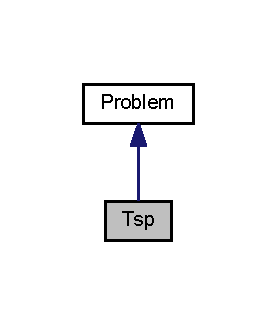
\includegraphics[width=133pt]{class_tsp__inherit__graph}
\end{center}
\end{figure}


Diagrama de colaboración para Tsp\+:
\nopagebreak
\begin{figure}[H]
\begin{center}
\leavevmode
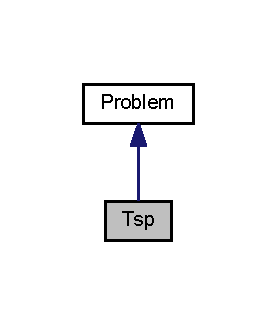
\includegraphics[width=133pt]{class_tsp__coll__graph}
\end{center}
\end{figure}
\subsection*{Métodos públicos}
\begin{DoxyCompactItemize}
\item 
\hyperlink{class_solution}{Solution} $\ast$ \hyperlink{class_tsp_ab37f446ab806d6f42e036a815a8eb0fb}{New\+Solution} ()
\begin{DoxyCompactList}\small\item\em Redefinicion del método para la clase \hyperlink{class_tsp}{Tsp}. \end{DoxyCompactList}\item 
double \hyperlink{class_tsp_a84ed21c114ae235e2c0f56177c164a0a}{Calcular\+Fitness} (\hyperlink{class_solution}{Solution} $\ast$sol)
\begin{DoxyCompactList}\small\item\em Redefinicion del método para la clase \hyperlink{class_tsp}{Tsp}. \end{DoxyCompactList}\item 
double \hyperlink{class_tsp_aae80b10d5d2b846a5f7d03fc44263ab2}{get\+Min\+Values\+Pos} (unsigned int pos)
\begin{DoxyCompactList}\small\item\em Redefinicion del método para la clase \hyperlink{class_tsp}{Tsp}. \end{DoxyCompactList}\item 
double \hyperlink{class_tsp_a5bdc7d7f407f9bc2084d77c971cb99ef}{get\+Max\+Values\+Pos} (unsigned int pos)
\begin{DoxyCompactList}\small\item\em Redefinicion del método para la clase \hyperlink{class_tsp}{Tsp}. \end{DoxyCompactList}\item 
unsigned int \hyperlink{class_tsp_a0f6463fc9e034a8c78bf4cac881df990}{get\+Dimension} ()
\begin{DoxyCompactList}\small\item\em Redefinicion del método para la clase \hyperlink{class_tsp}{Tsp}. \end{DoxyCompactList}\item 
bool \hyperlink{class_tsp_a9a77be6018464e5380296fa8decc36ac}{Es\+Dinamico} ()
\begin{DoxyCompactList}\small\item\em Redefinicion del método para la clase \hyperlink{class_tsp}{Tsp}. \end{DoxyCompactList}\item 
void \hyperlink{class_tsp_a15c1d7f52f3d6ce233d86beda80eabf4}{step} (std\+::vector$<$ std\+::vector$<$ double $>$ $>$, int)
\begin{DoxyCompactList}\small\item\em Redefinicion del método para la clase \hyperlink{class_tsp}{Tsp}. \end{DoxyCompactList}\item 
\hypertarget{class_tsp_a499348dd3e9939f2cf04603382735285}{vector$<$ vector$<$ double $>$ $>$ {\bfseries read\+T\+S\+P\+Problem\+File} (string filename)}\label{class_tsp_a499348dd3e9939f2cf04603382735285}

\end{DoxyCompactItemize}
\subsection*{Otros miembros heredados}


\subsection{Documentación de las funciones miembro}
\hypertarget{class_tsp_a84ed21c114ae235e2c0f56177c164a0a}{\index{Tsp@{Tsp}!Calcular\+Fitness@{Calcular\+Fitness}}
\index{Calcular\+Fitness@{Calcular\+Fitness}!Tsp@{Tsp}}
\subsubsection[{Calcular\+Fitness}]{\setlength{\rightskip}{0pt plus 5cm}double Tsp\+::\+Calcular\+Fitness (
\begin{DoxyParamCaption}
\item[{{\bf Solution} $\ast$}]{sol}
\end{DoxyParamCaption}
)\hspace{0.3cm}{\ttfamily [virtual]}}}\label{class_tsp_a84ed21c114ae235e2c0f56177c164a0a}


Redefinicion del método para la clase \hyperlink{class_tsp}{Tsp}. 


\begin{DoxyParams}{Parámetros}
{\em sol} & Puntero a la solución, que se desea determinar su fitness en la subclase \hyperlink{class_tsp}{Tsp} \\
\hline
\end{DoxyParams}


Implementa \hyperlink{class_problem_adc6176be667576d08cf3e89b65e905f4}{Problem}.

\hypertarget{class_tsp_a9a77be6018464e5380296fa8decc36ac}{\index{Tsp@{Tsp}!Es\+Dinamico@{Es\+Dinamico}}
\index{Es\+Dinamico@{Es\+Dinamico}!Tsp@{Tsp}}
\subsubsection[{Es\+Dinamico}]{\setlength{\rightskip}{0pt plus 5cm}bool Tsp\+::\+Es\+Dinamico (
\begin{DoxyParamCaption}
{}
\end{DoxyParamCaption}
)\hspace{0.3cm}{\ttfamily [virtual]}}}\label{class_tsp_a9a77be6018464e5380296fa8decc36ac}


Redefinicion del método para la clase \hyperlink{class_tsp}{Tsp}. 

\begin{DoxyReturn}{Devuelve}
Retorna valor del tipo booleano, con la respuesta de si es o no, dinámico el problema 
\end{DoxyReturn}


Implementa \hyperlink{class_problem_a481dc3e5869cf95b3c539d552e8eeb50}{Problem}.

\hypertarget{class_tsp_a0f6463fc9e034a8c78bf4cac881df990}{\index{Tsp@{Tsp}!get\+Dimension@{get\+Dimension}}
\index{get\+Dimension@{get\+Dimension}!Tsp@{Tsp}}
\subsubsection[{get\+Dimension}]{\setlength{\rightskip}{0pt plus 5cm}unsigned int Tsp\+::get\+Dimension (
\begin{DoxyParamCaption}
{}
\end{DoxyParamCaption}
)\hspace{0.3cm}{\ttfamily [virtual]}}}\label{class_tsp_a0f6463fc9e034a8c78bf4cac881df990}


Redefinicion del método para la clase \hyperlink{class_tsp}{Tsp}. 

\begin{DoxyReturn}{Devuelve}
Retorna valor del tipo entero sin signo, con el valor de la dimensión del problema 
\end{DoxyReturn}


Implementa \hyperlink{class_problem_a6f72067600654aef0767bce95c4eacdd}{Problem}.

\hypertarget{class_tsp_a5bdc7d7f407f9bc2084d77c971cb99ef}{\index{Tsp@{Tsp}!get\+Max\+Values\+Pos@{get\+Max\+Values\+Pos}}
\index{get\+Max\+Values\+Pos@{get\+Max\+Values\+Pos}!Tsp@{Tsp}}
\subsubsection[{get\+Max\+Values\+Pos}]{\setlength{\rightskip}{0pt plus 5cm}double Tsp\+::get\+Max\+Values\+Pos (
\begin{DoxyParamCaption}
\item[{unsigned int}]{pos}
\end{DoxyParamCaption}
)\hspace{0.3cm}{\ttfamily [virtual]}}}\label{class_tsp_a5bdc7d7f407f9bc2084d77c971cb99ef}


Redefinicion del método para la clase \hyperlink{class_tsp}{Tsp}. 


\begin{DoxyParams}{Parámetros}
{\em pos} & Posición de la coordenada\\
\hline
\end{DoxyParams}
\begin{DoxyReturn}{Devuelve}
Retorna valor del tipo double, con el valor de esa coordenada para los máximos valores 
\end{DoxyReturn}


Implementa \hyperlink{class_problem_a2ffe7de8658a25398d6a21dd1b2edfcb}{Problem}.

\hypertarget{class_tsp_aae80b10d5d2b846a5f7d03fc44263ab2}{\index{Tsp@{Tsp}!get\+Min\+Values\+Pos@{get\+Min\+Values\+Pos}}
\index{get\+Min\+Values\+Pos@{get\+Min\+Values\+Pos}!Tsp@{Tsp}}
\subsubsection[{get\+Min\+Values\+Pos}]{\setlength{\rightskip}{0pt plus 5cm}double Tsp\+::get\+Min\+Values\+Pos (
\begin{DoxyParamCaption}
\item[{unsigned int}]{pos}
\end{DoxyParamCaption}
)\hspace{0.3cm}{\ttfamily [virtual]}}}\label{class_tsp_aae80b10d5d2b846a5f7d03fc44263ab2}


Redefinicion del método para la clase \hyperlink{class_tsp}{Tsp}. 


\begin{DoxyParams}{Parámetros}
{\em pos} & Indica la posición de la coordenada\\
\hline
\end{DoxyParams}
\begin{DoxyReturn}{Devuelve}
Retorna valor del tipo double, con el valor de esa coordenada para los mínimos valores 
\end{DoxyReturn}


Implementa \hyperlink{class_problem_ad6a122249b93487f91a64837a056fa75}{Problem}.

\hypertarget{class_tsp_ab37f446ab806d6f42e036a815a8eb0fb}{\index{Tsp@{Tsp}!New\+Solution@{New\+Solution}}
\index{New\+Solution@{New\+Solution}!Tsp@{Tsp}}
\subsubsection[{New\+Solution}]{\setlength{\rightskip}{0pt plus 5cm}{\bf Solution} $\ast$ Tsp\+::\+New\+Solution (
\begin{DoxyParamCaption}
{}
\end{DoxyParamCaption}
)\hspace{0.3cm}{\ttfamily [virtual]}}}\label{class_tsp_ab37f446ab806d6f42e036a815a8eb0fb}


Redefinicion del método para la clase \hyperlink{class_tsp}{Tsp}. 

\begin{DoxyReturn}{Devuelve}
Retorna puntero del tipo \hyperlink{class_solution}{Solution}, con una nueva solución relacionada con la codificación en particular para el problema, específicamente Solution\+R\+N 
\end{DoxyReturn}


Implementa \hyperlink{class_problem_a4b9787b3945dbec08e402c0cfd0f646b}{Problem}.

\hypertarget{class_tsp_a15c1d7f52f3d6ce233d86beda80eabf4}{\index{Tsp@{Tsp}!step@{step}}
\index{step@{step}!Tsp@{Tsp}}
\subsubsection[{step}]{\setlength{\rightskip}{0pt plus 5cm}void Tsp\+::step (
\begin{DoxyParamCaption}
\item[{std\+::vector$<$ std\+::vector$<$ double $>$ $>$}]{, }
\item[{int}]{}
\end{DoxyParamCaption}
)\hspace{0.3cm}{\ttfamily [virtual]}}}\label{class_tsp_a15c1d7f52f3d6ce233d86beda80eabf4}


Redefinicion del método para la clase \hyperlink{class_tsp}{Tsp}. 


\begin{DoxyParams}{Parámetros}
{\em datos} & Arreglo de arreglo con valores de todas las plantas presentes en el patio \\
\hline
{\em iter} & Numero de la iteracion actual \\
\hline
\end{DoxyParams}


Implementa \hyperlink{class_problem_a0c7025eb5127b1eda7988cceadc00da6}{Problem}.



La documentación para esta clase fue generada a partir de los siguientes ficheros\+:\begin{DoxyCompactItemize}
\item 
T\+S\+P\+\_\+\+P\+E\+R\+M/Tsp.\+h\item 
T\+S\+P\+\_\+\+P\+E\+R\+M/Tsp.\+cpp\end{DoxyCompactItemize}

%--- End generated contents ---

% Index
\newpage
\phantomsection
\addcontentsline{toc}{chapter}{Índice}
\printindex

\end{document}
